\documentclass{beamer}

%\usepackage[utf8x]{inputenc}
\usepackage{graphicx}
\usepackage{hyperref}
\usepackage{xspace}
\usepackage{amsmath}
\usetheme{Madrid}

\definecolor{pink}{rgb}{1.0,.8,.8}
\definecolor{hotpink}{cmyk}{0.0,0.8,0,0.2}
\definecolor{softred}{rgb}{.9,.7,.7}
\definecolor{darkred}{rgb}{.8,.1,.1}
\definecolor{purple}{rgb}{.7,.0,.7}
\definecolor{darkgreen}{rgb}{.1,.45,.1}
\definecolor{lightblue}{rgb}{0.3,0.3,1.0}
\definecolor{grey}{rgb}{.5,.5,.5}


\newcommand{\darkred}[1]{\textcolor{darkred}{#1}}
\newcommand{\darkgreen}[1]{\textcolor{darkgreen}{#1}}
\newcommand{\hotpink}[1]{\textcolor{hotpink}{#1}}
\newcommand{\lightblue}[1]{\textcolor{lightblue}{#1}}
\newcommand{\blue}[1]{\textcolor{blue}{#1}}
\newcommand{\red}[1]{\textcolor{red}{#1}}
\newcommand{\green}[1]{\textcolor{green}{#1}}
\newcommand{\purple}[1]{\textcolor{purple}{#1}}
\newcommand{\grey}[1]{\textcolor{grey}{#1}}
\newcommand{\MetDeltaPhi}{\Delta\phi(\MET, \rm{lepton, jet})}
\newcommand{\MET}{\mbox{$E\kern-0.50em\raise0.10ex\hbox{/}_{T}$}}
\newcommand{\met}{\ensuremath{E_T^{miss}}\xspace}
\newcommand{\metrel}{\ensuremath{E_{T}^{miss,~\mathrm{Rel}}}\xspace} 
\newcommand{\tmet}{\ensuremath{E_{T}^{miss,~\mathrm{Track}}}\xspace} 
\newcommand{\ptll}{\ensuremath{p_{T}^{\ell\ell}}\xspace} 
\newcommand{\ptg}{\ensuremath{p_{T}^{\gamma}}\xspace} 
\newcommand{\ptZ}{\ensuremath{p_{T}^{Z}}\xspace} 
\newcommand{\METsig}{\MET_{\mathrm{sig}}}
\newcommand{\delPhiMet}{\min{\Delta\phi(\MET,l\mathrm{~or~jet}))}} 
\newcommand{\dphill}{\ensuremath{\Delta\phi_{\ell\ell}}} 
\newcommand{\SumEt}{\sum{E_{T}}}
\newcommand{\nunubar}{\nu \overline{\nu}}
\newcommand{\ttbar}{t \overline{t}}
\newcommand{\ppbar}{p \overline{p}}
\newcommand{\qqbar}{q \overline{q}}
\newcommand{\bbbar}{b \overline{b}}
\newcommand{\epem}{ e^+e^-}
\newcommand{\pt}{\ensuremath{p_{T}}\xspace}
\newcommand{\HWW}{H\rightarrow WW}
\newcommand{\BR}[1]{{\cal{B}} (#1)}
\newcommand{\zzllnunu}{\ensuremath{ZZ\to\ell\ell\nu\nu}\;}

\newcommand {\Dzero} {D\O\ }

\newcommand {\rmfrac}[2]{ $\frac{\mathrm{#1}}{\mathrm{#2}}$ }

\newcommand{\bc}{\begin{columns}}
\newcommand{\ec}{\end{columns}}
\newcommand{\fr}[2]{\begin{frame} \frametitle{#1} #2 \end{frame} }


\newcommand{\figbox}[5][]{
   \parbox{#2\textwidth}{
   \centering
   \includegraphics[#1,width=#3\textwidth]{#4}
   \ifthenelse{ \equal{}{#5} } {} {\\ #5}
}} 

\newcommand{\figboxv}[4]{
   \parbox{#1\textwidth}{
   \begin{center}
   \includegraphics[height=#2\textwidth]{#3}   
   \ifthenelse{ \equal{}{#4} } {} {
     \vspace{-0.35cm}
     \begin{center}
       #4
     \end{center}
   }
   \end{center}
}} 



\title[ WgamgamUpdtes ]
{ A few studies } 

\author[Josh Kunkle]
  {Josh Kunkle}

\institute[UMD]{University of Maryland}

\date[February 27, 2014] % (optional)
{ 
  \vspace{0.5cm} \begin{center}
\includegraphics[width=0.3\textwidth]{../UMDLogo.pdf}\end{center}
  \vspace{0.5cm}
}

\begin{document}

\maketitle

\fr{ Outline } {

    \begin{itemize}
        \item Photon overlap removal between MC samples
        \item Lepton momentum corrections
        \item Second lepton veto
        \item Three photon events
    \end{itemize}

}

\fr{ Photon overlap between MC samples } {

    The phase space of photon emission overlaps between MC samples

    \begin{columns}
        \column{0.2\textwidth}
            \begin{itemize}
                \item Wjets
                \item W$\gamma$
                \item W$\gamma\gamma$
            \end{itemize}

            \column{0.2\textwidth}

            \begin{itemize}
                \item Zjets
                \item Z$\gamma$
            \end{itemize}

            \column{0.5\textwidth}

    \end{columns}

    \begin{itemize}
        \item The samples that add a photon require the emission of at least one additional hard photon
        \item Therefore we must veto events in the samples without the filter that have a hard photon
        \item Use mcParentage to determine if parent is lepton or QCD if(mcParentage \& 0x12) == 0x12 ) n\_hard\_photons++
        \item In Wjets,Zjets require 0 hard photons, in W$\gamma$ require 1 hard photon
    \end{itemize}
}

\fr{ Check overlap removal in 2lepton + photon CR } {

    \scriptsize

    \bc
        \column{0.5\textwidth}
        $e e \gamma$

        before

        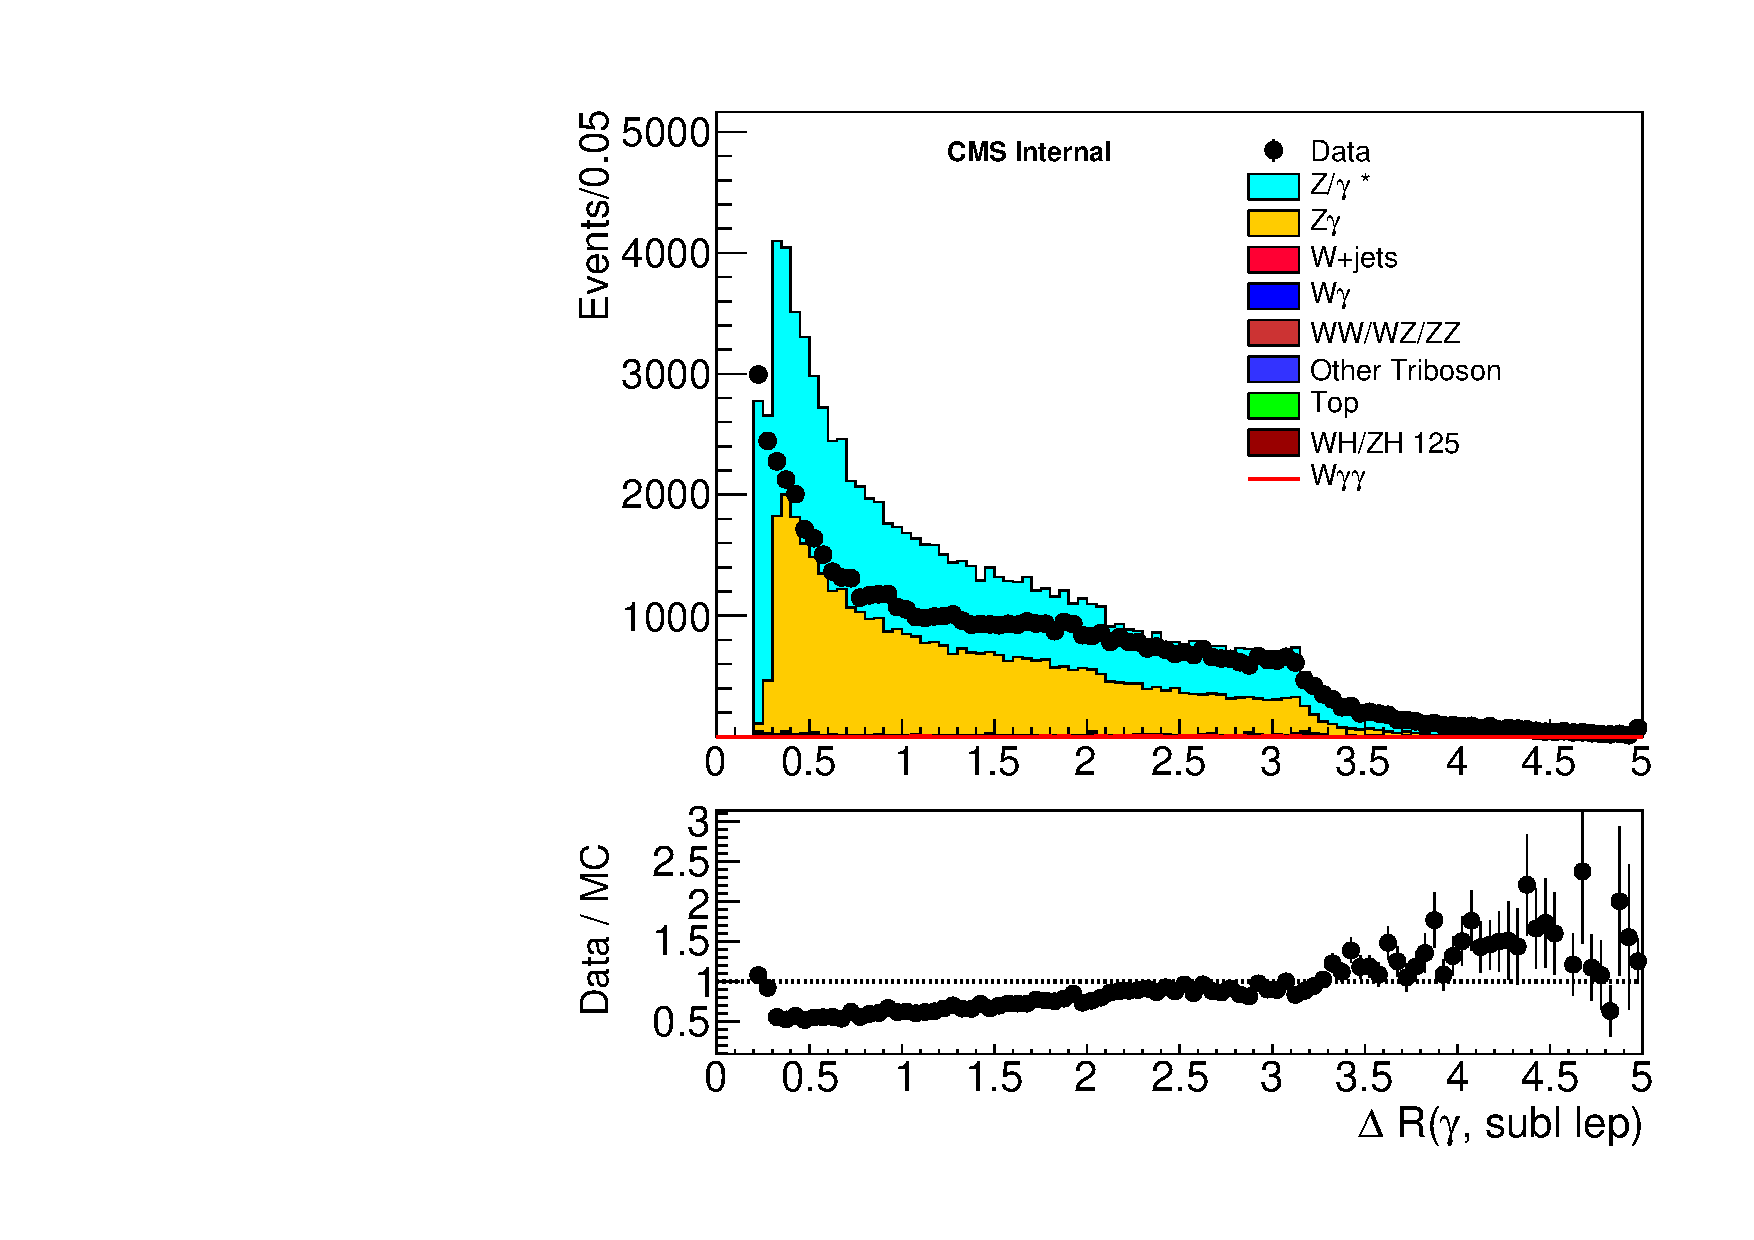
\includegraphics[width=0.6\textwidth]{Plots/m_leplep_elelph_phsubllepDR.pdf}

        after

        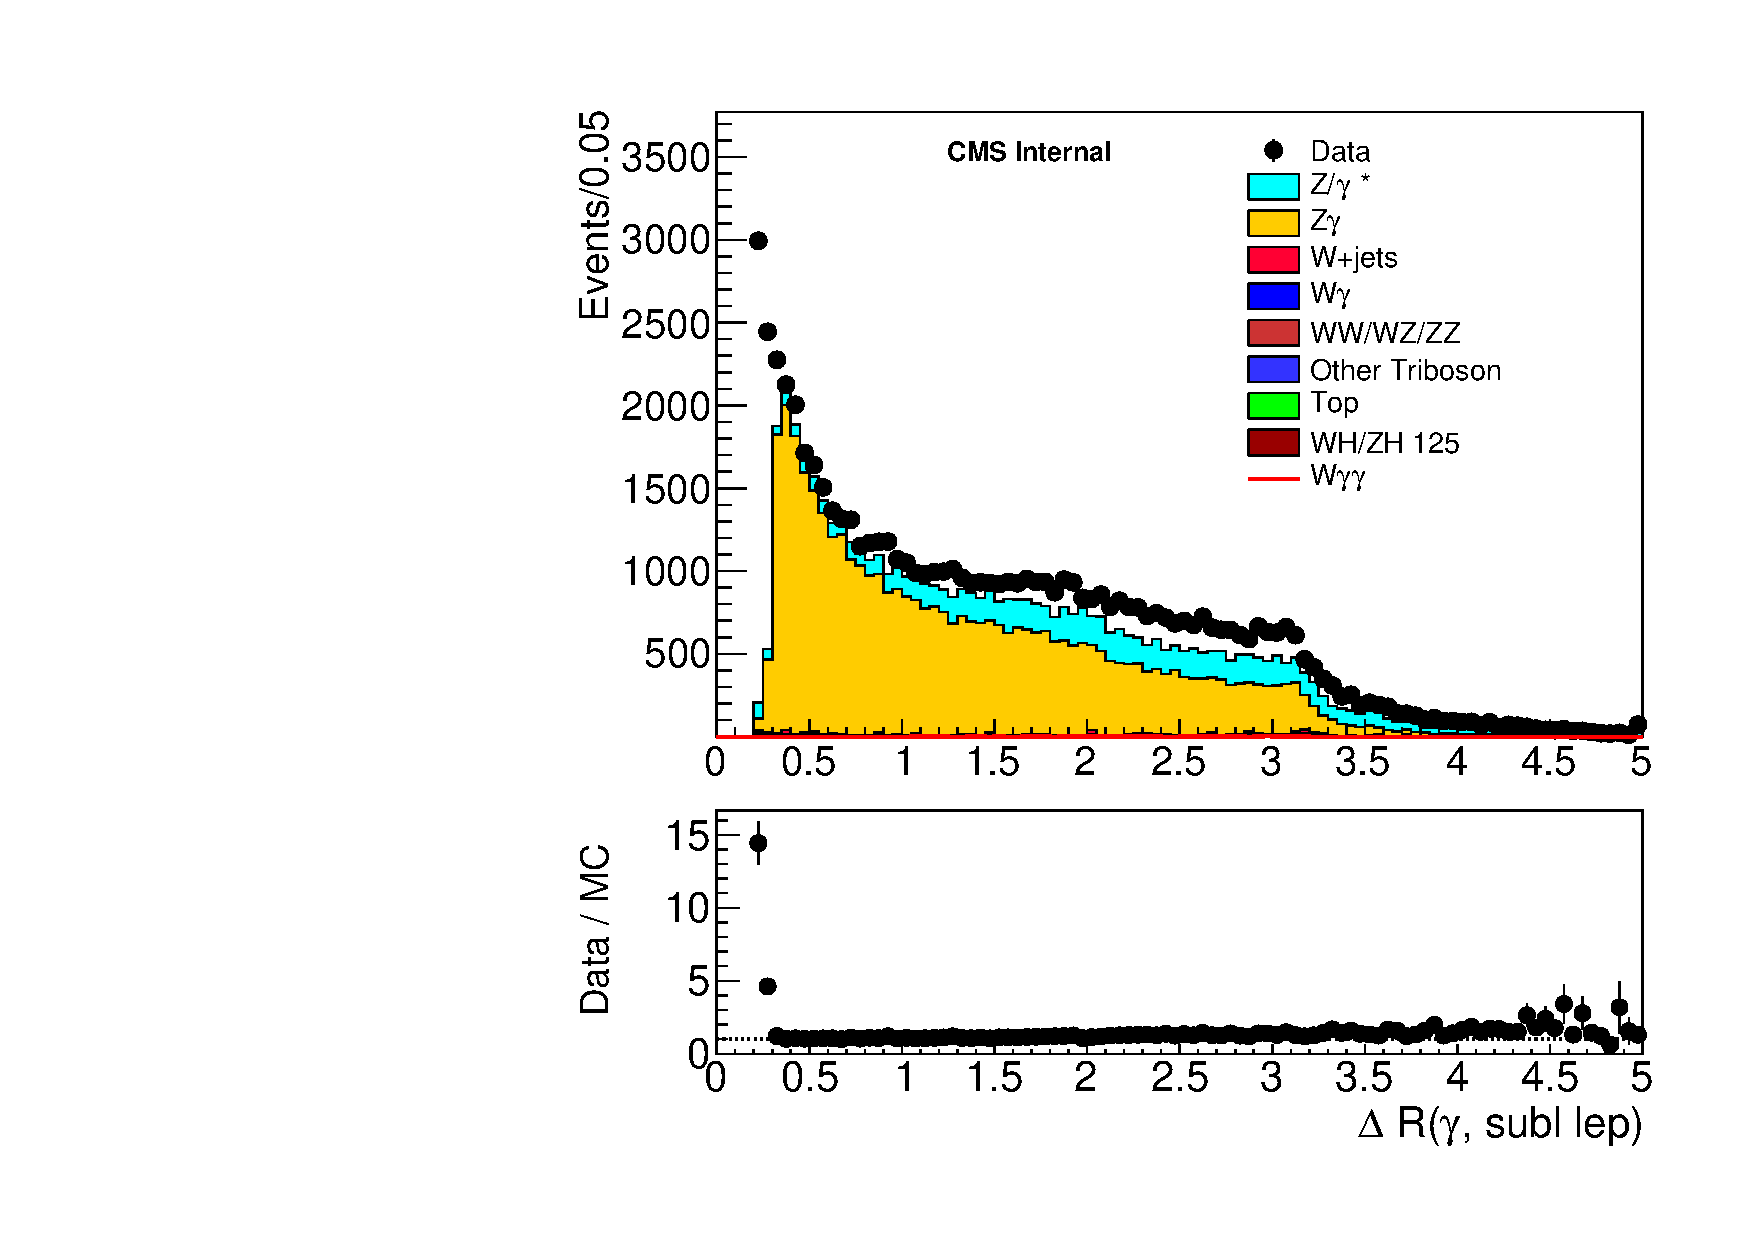
\includegraphics[width=0.6\textwidth]{Plots/m_leplep_elelph_phsubllepDR_oldOlap.pdf}

        \column{0.5\textwidth}

        $\mu\mu \gamma$

            before
            
        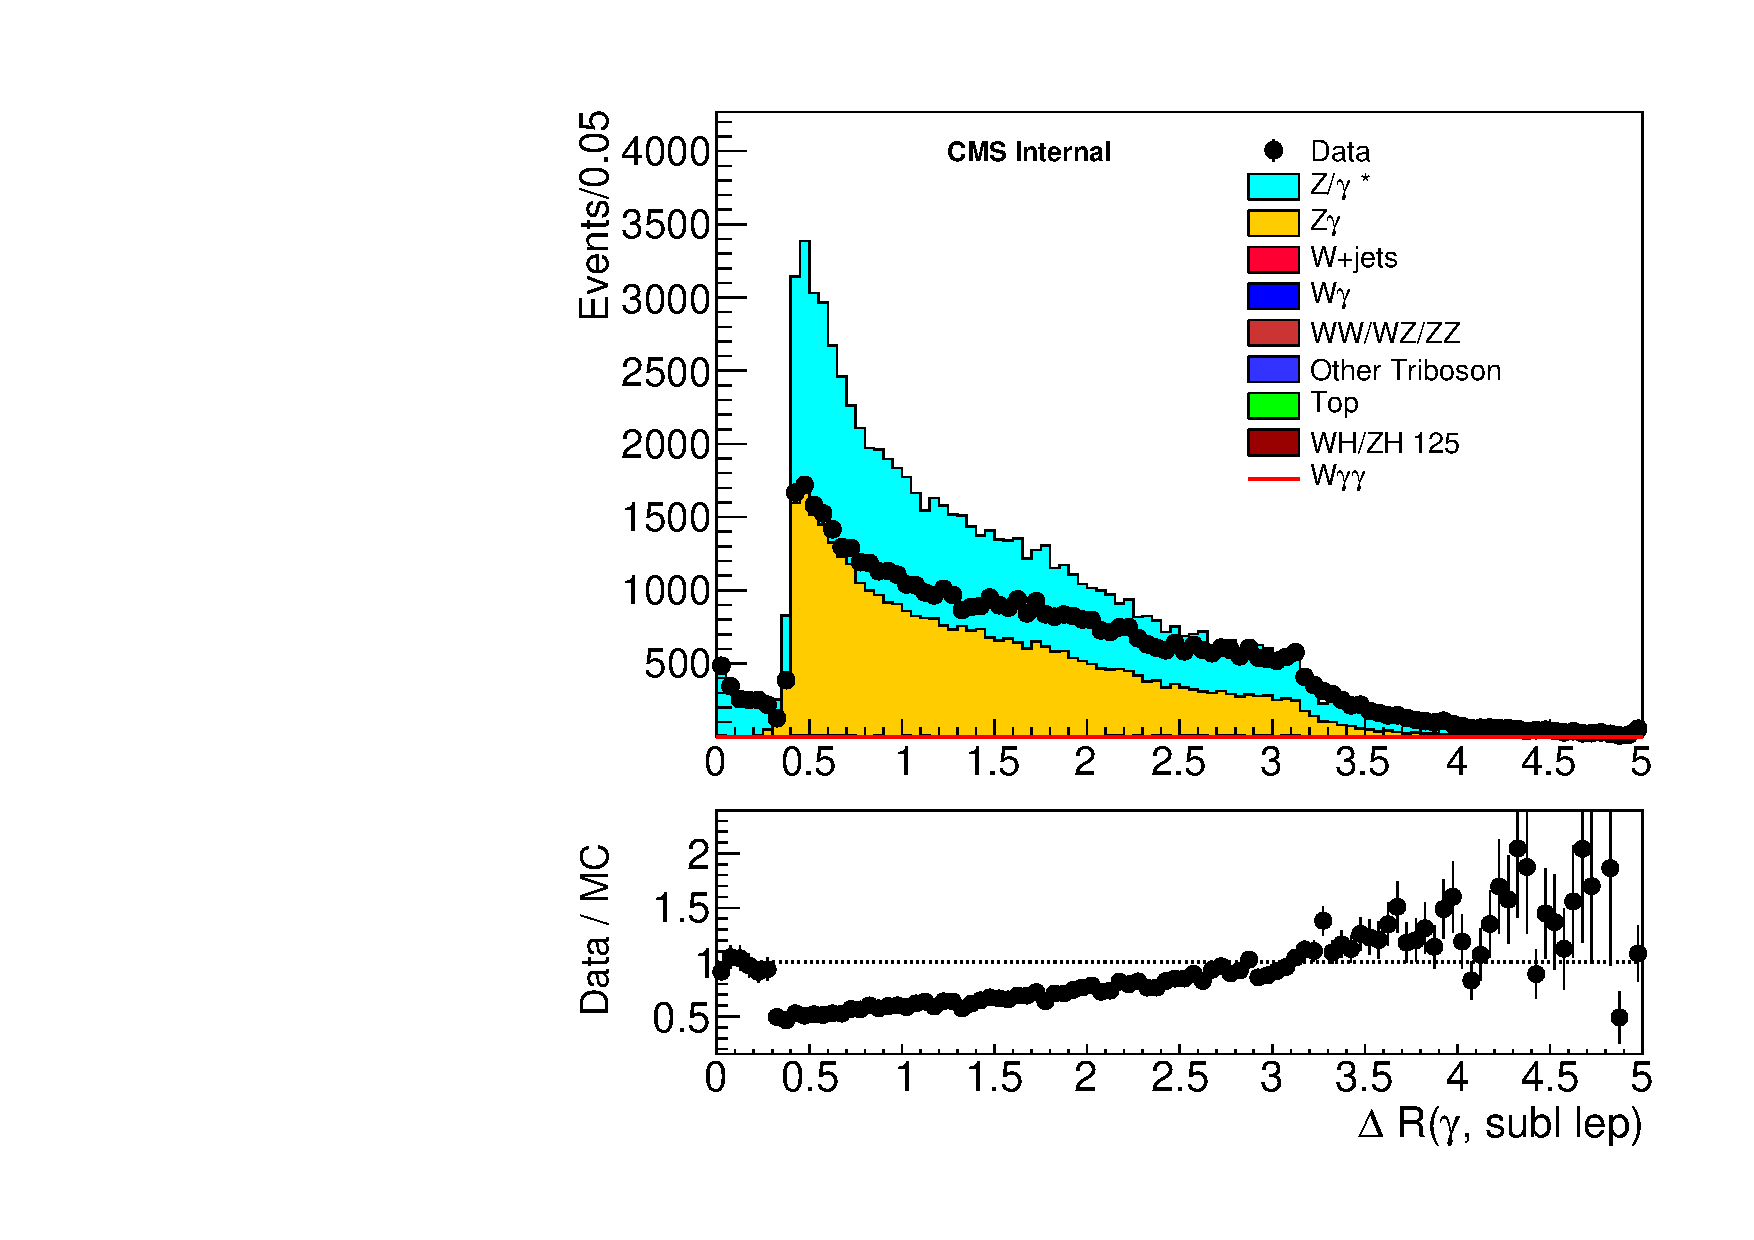
\includegraphics[width=0.6\textwidth]{Plots/m_leplep_mumuph_phsubllepDR.pdf}

        after
        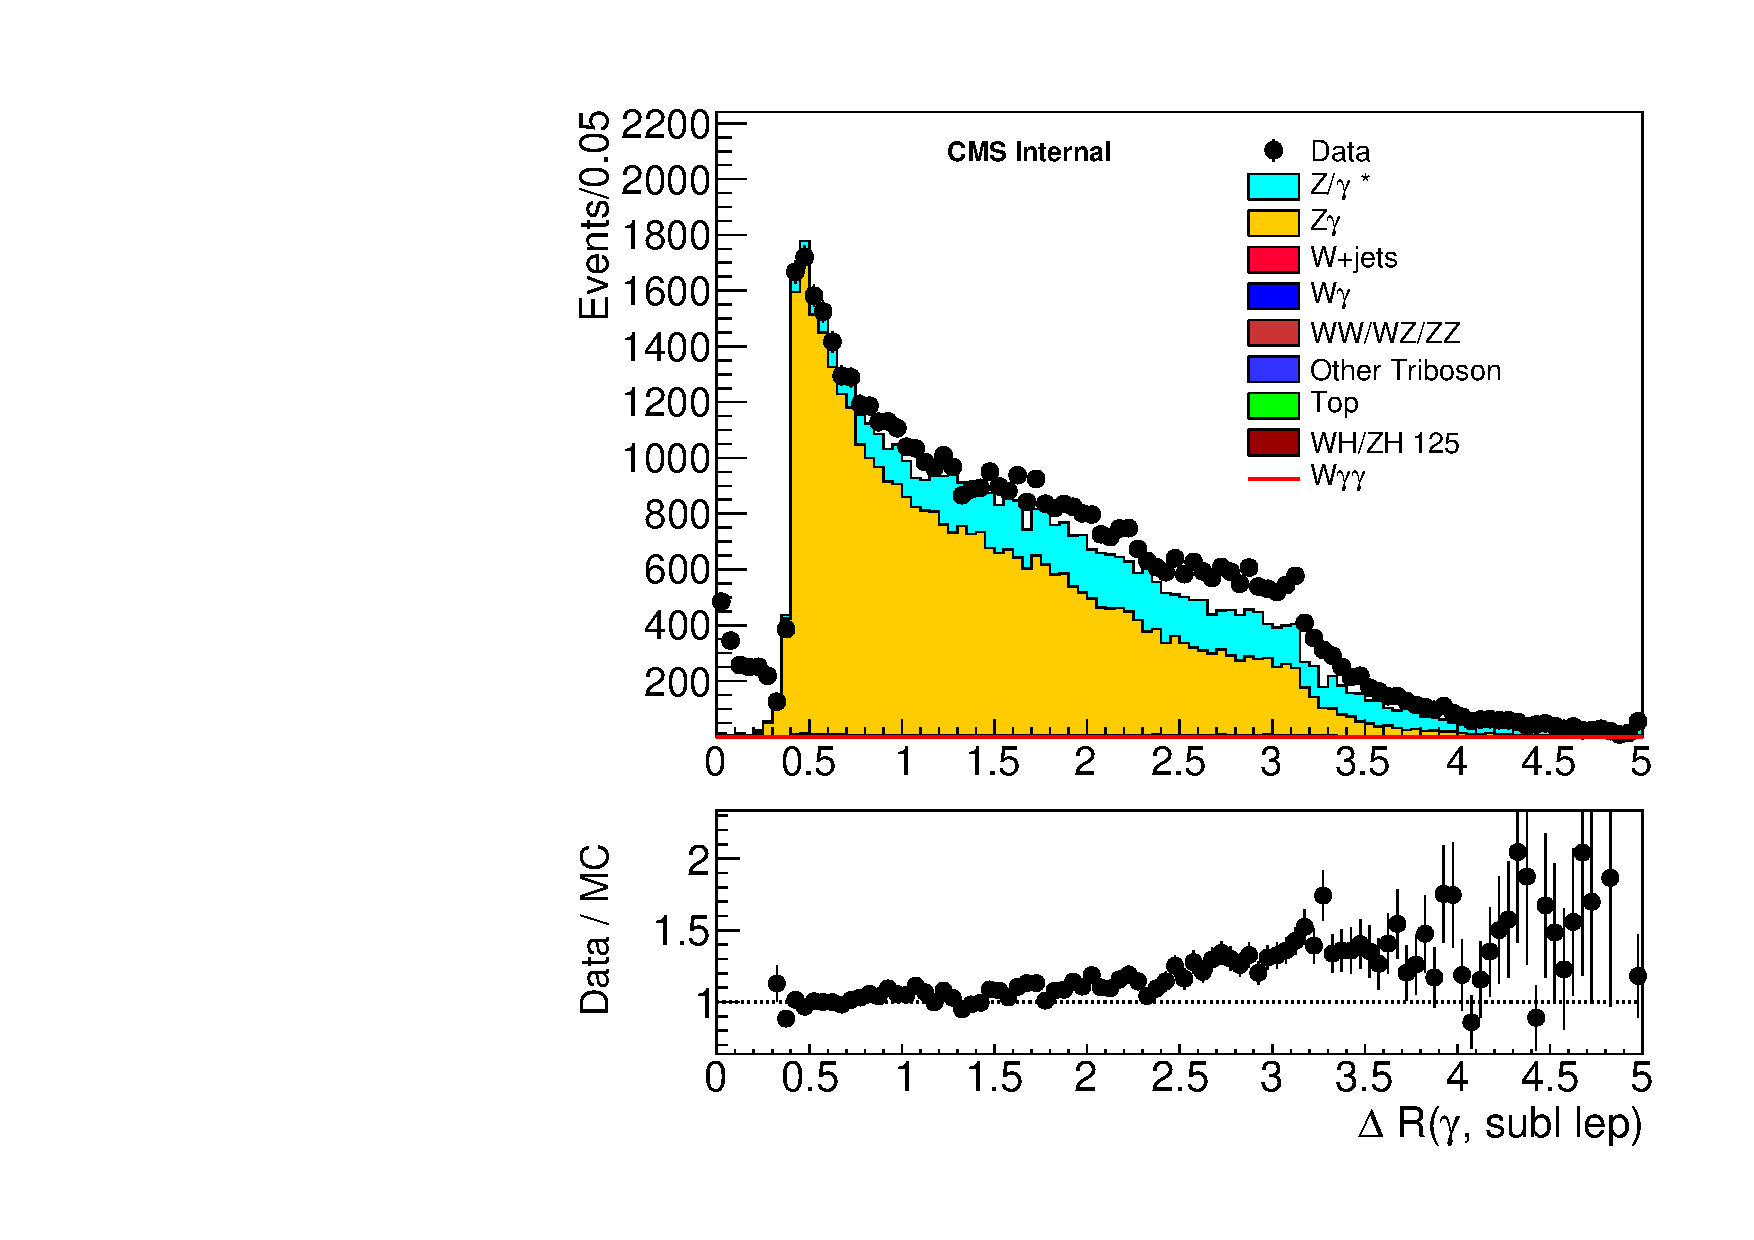
\includegraphics[width=0.6\textwidth]{Plots/m_leplep_mumuph_phsubllepDR_oldOlap.pdf}

    \ec

}

\fr{ Modification of hard photon requirement } {

    \bc
        \column{0.5\textwidth}
        \begin{itemize}
            \item From the previous slide, its clear that we should add a $\Delta R$ cut to the hard photon requirement
            \item In the Zg sample, the generator level $\Delta R$ cut is 0.3
        \end{itemize}
     
        \column{0.5\textwidth}
        
        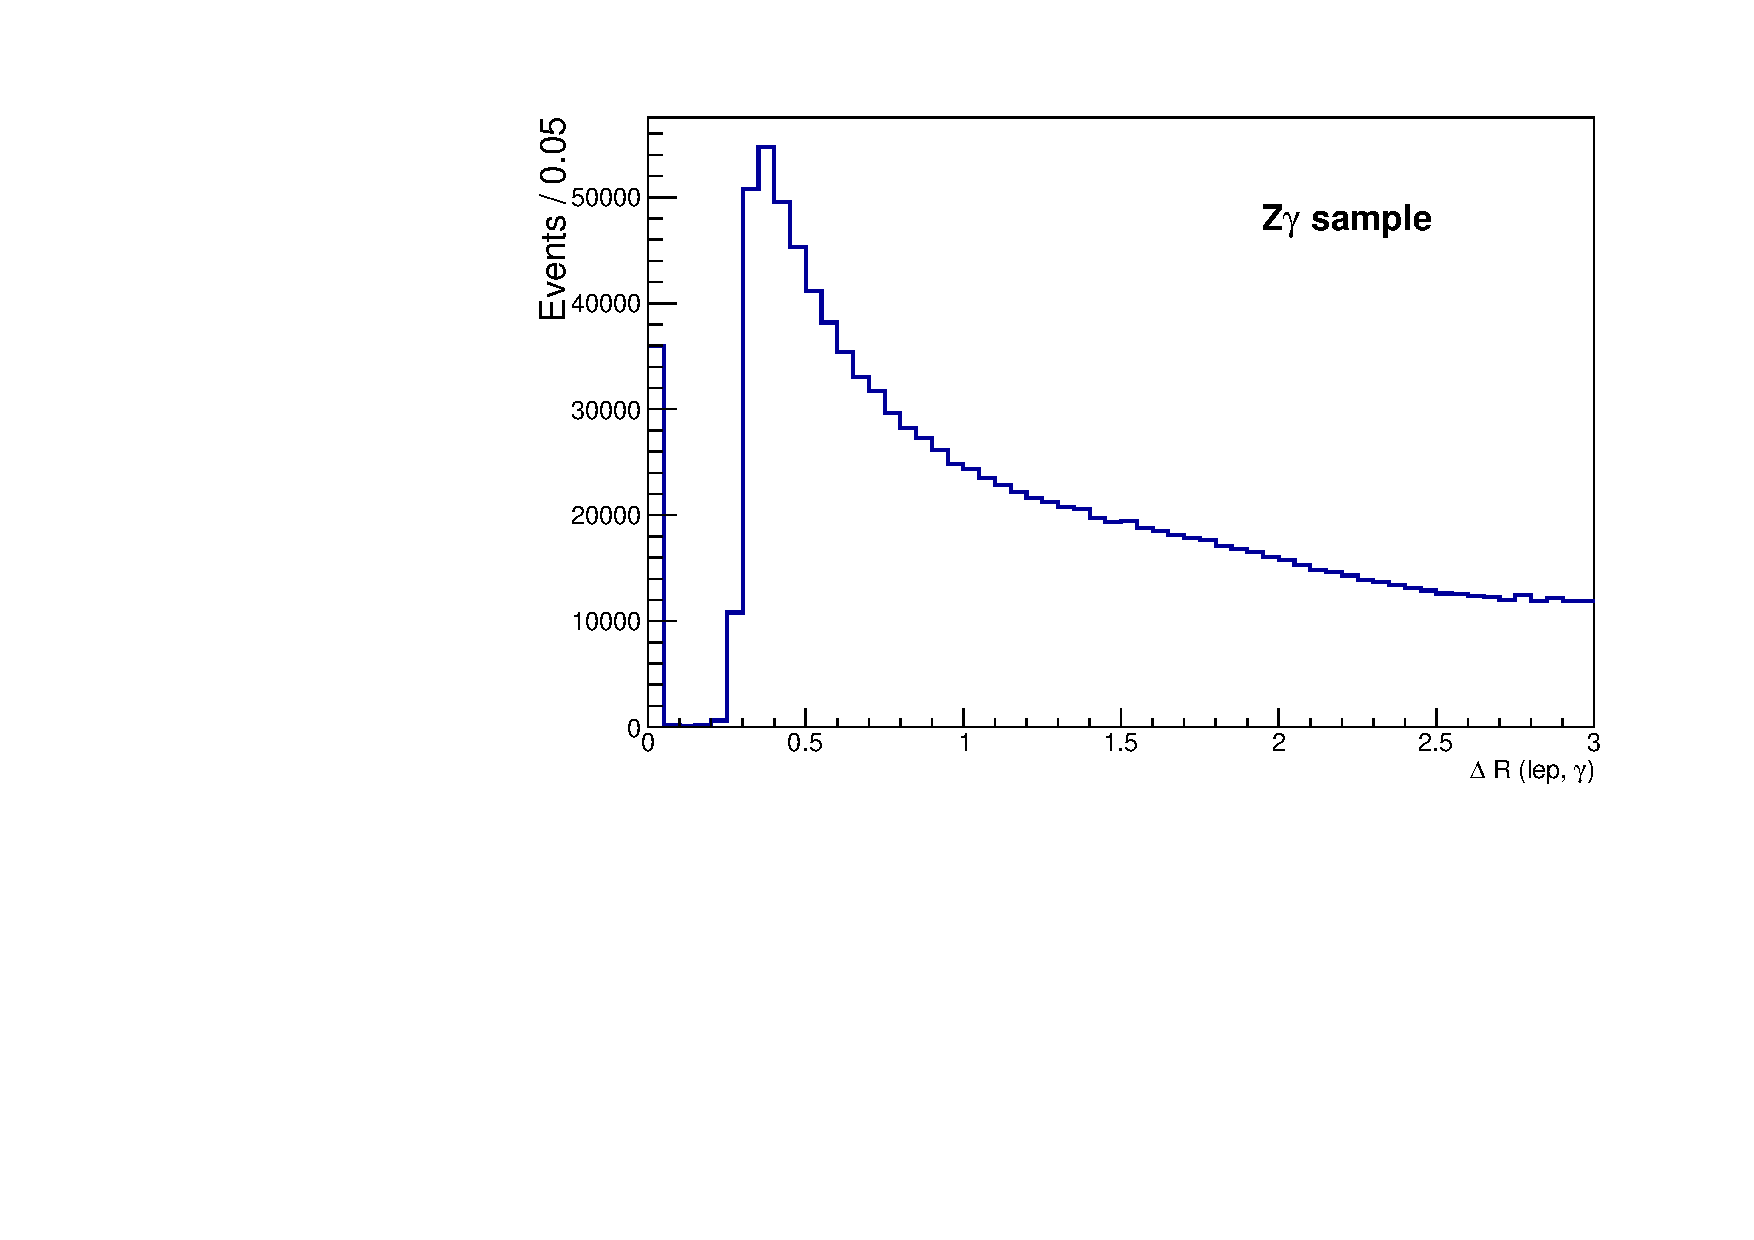
\includegraphics[width=0.8\textwidth]{Plots/LepPhotDRTruthZg.pdf}

    \ec

    \begin{itemize}
        \item Procedure :
        \begin{itemize} 
            \item Identify a photon using mcParentage as before
            \item Find the parent particle (usually a lepton, sometimes a pion) by PID
            \item A direct index link is not available in the ntuples, so a particle with matching PID may not be the mother
            \item Calculate the $\Delta R$ with all potential mothers.  If none are less than 0.3, this is a hard photon
        \end{itemize}
    \end{itemize}

}

\fr{ After modification } {

    MC agrees better wit data at low $\Delta R$

    \bc
        \column{0.5\textwidth}
    
        $e e \gamma$

        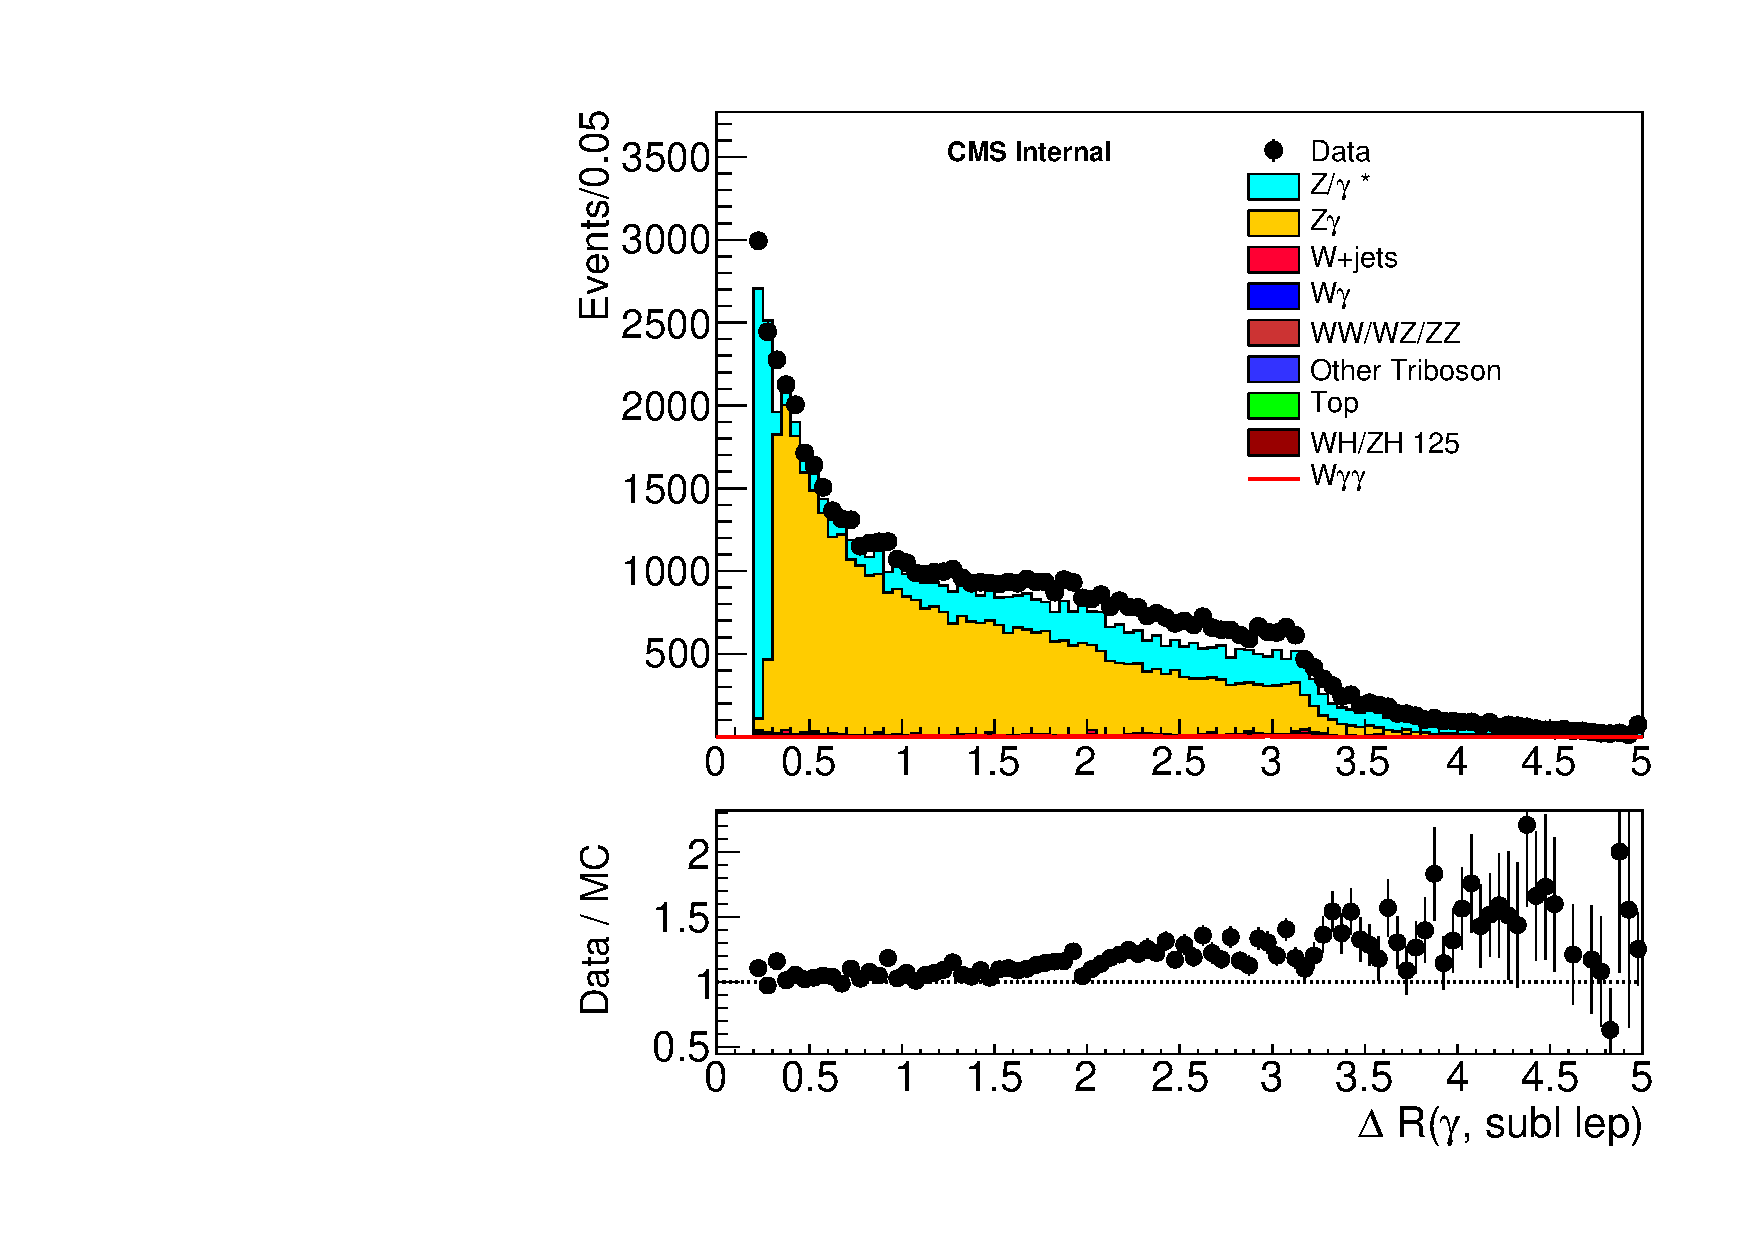
\includegraphics[width=0.8\textwidth]{Plots/m_leplep_elelph_phsubllepDR_newOlap.pdf}

        \column{0.5\textwidth}

        $\mu\mu \gamma$

        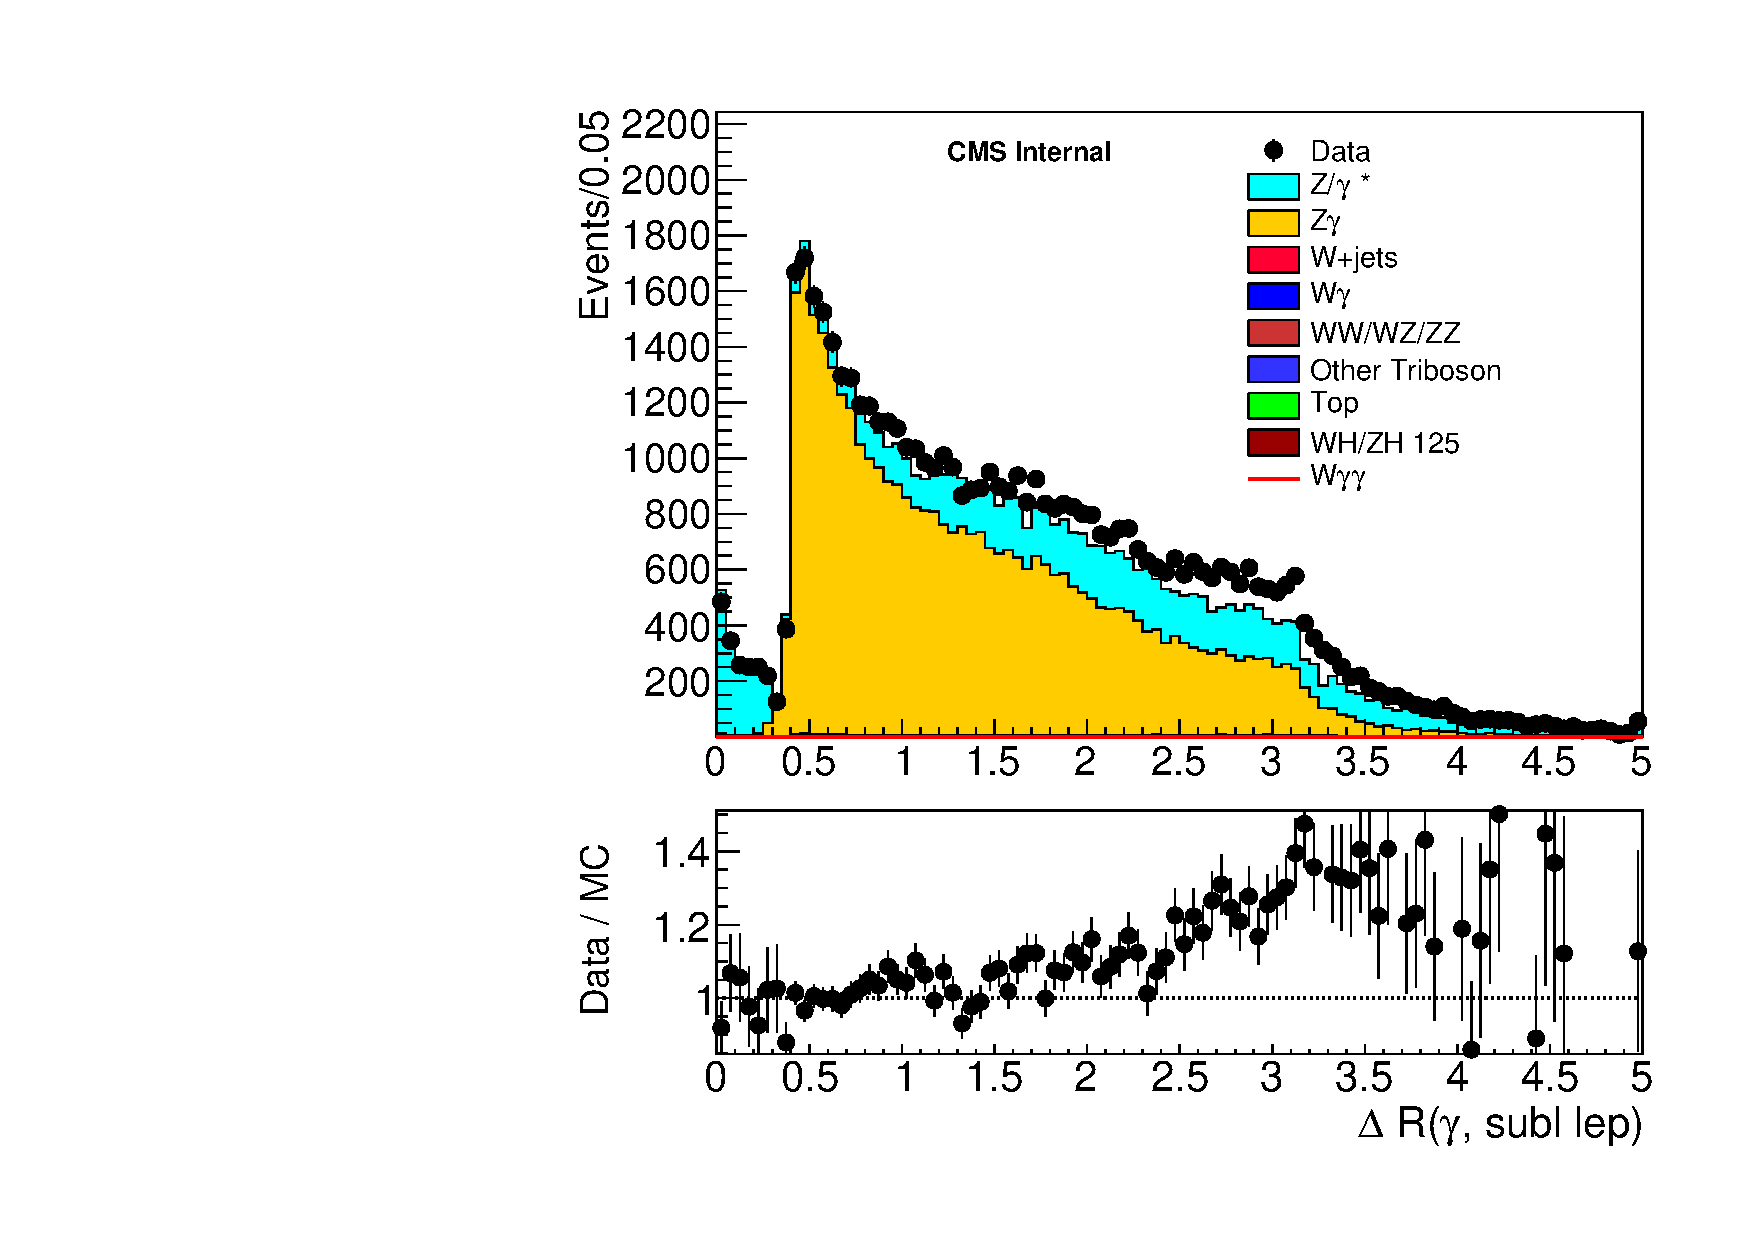
\includegraphics[width=0.8\textwidth]{Plots/m_leplep_mumuph_phsubllepDR_newOlap.pdf}

    \ec
}

\fr{ Check corrected lepton momentum in 2 lepton CR } {

    \begin{itemize}
        \item Applying corrections to electron and muon momenta in MC
        \item Following procedures linked on twiki
    \end{itemize}

    \bc
        \column{0.5\textwidth}
        Electrons
   
        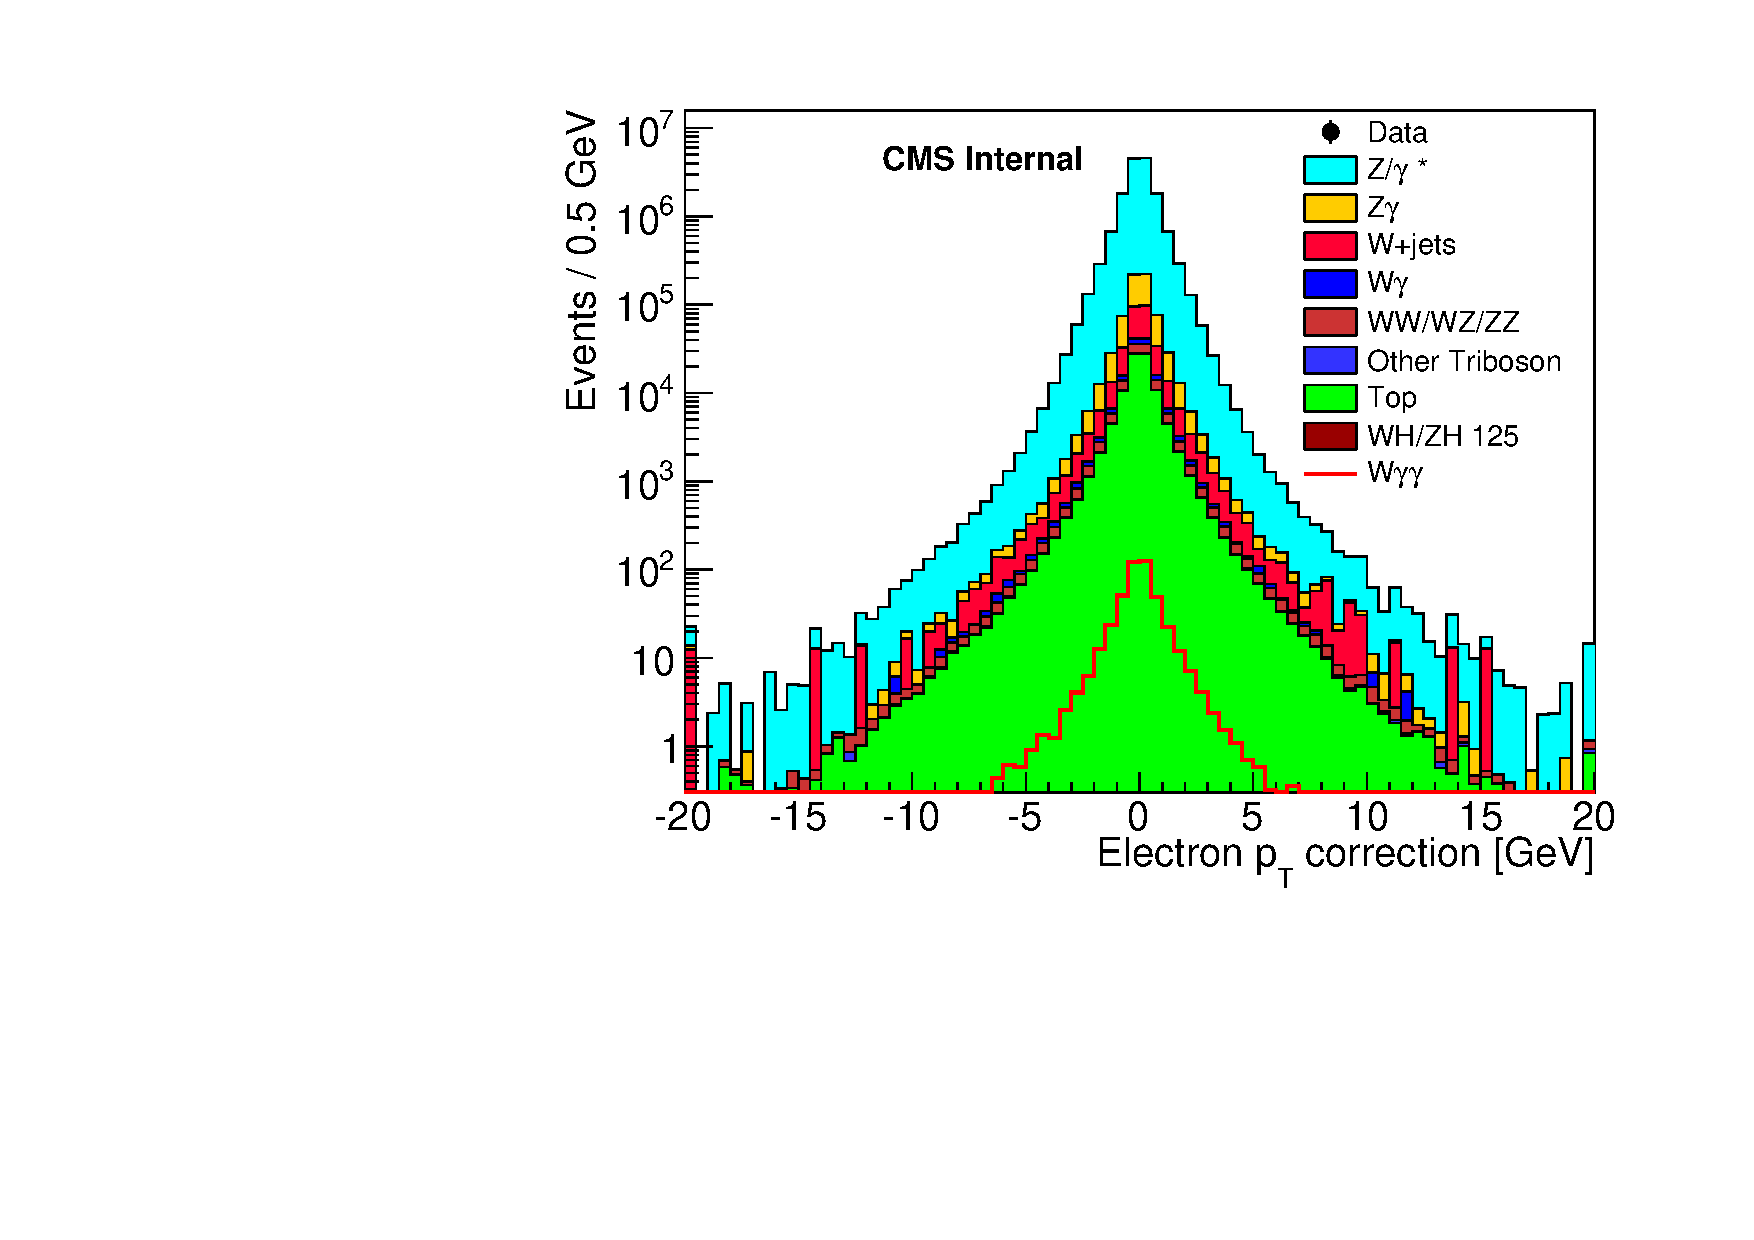
\includegraphics[width=0.8\textwidth]{Plots/electronPtCorrection.pdf}

        \column{0.5\textwidth}
        Muons

        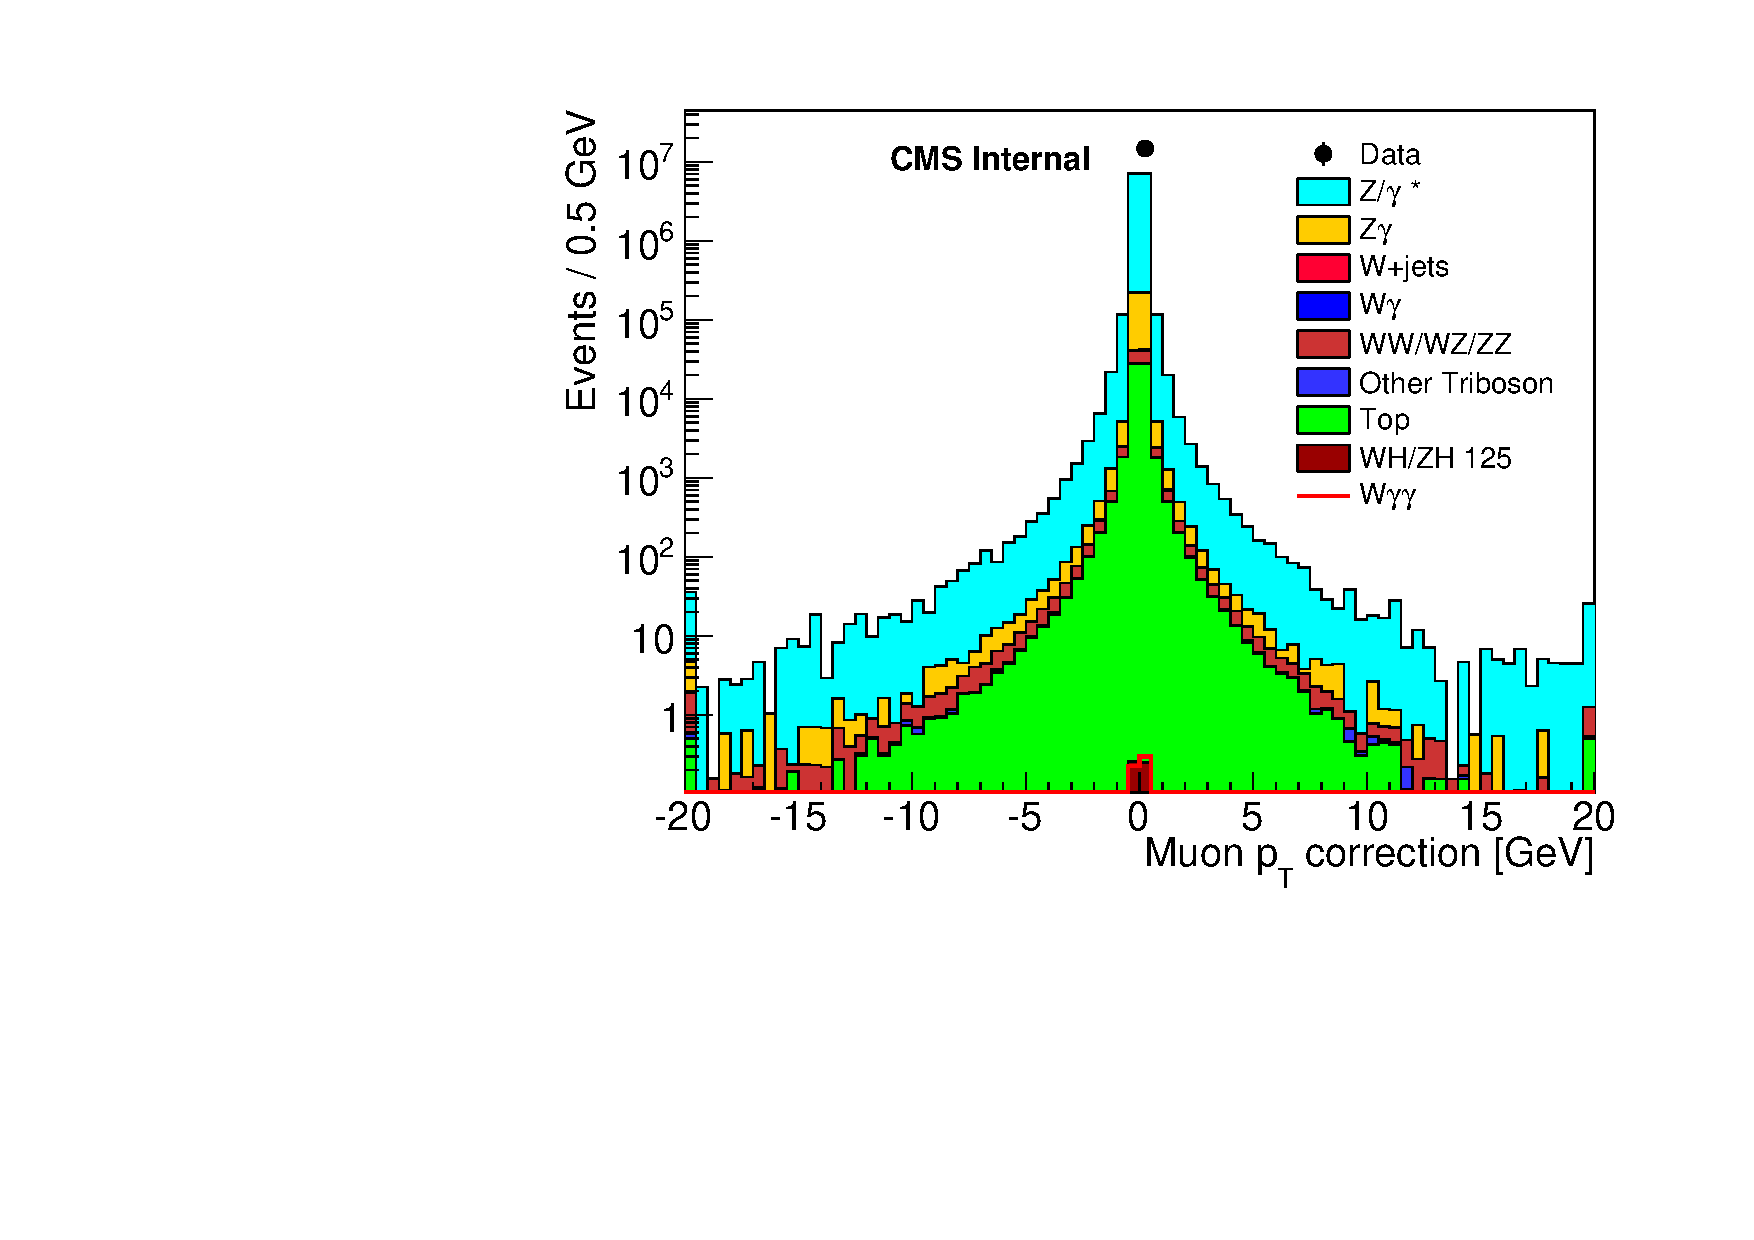
\includegraphics[width=0.8\textwidth]{Plots/muonPtCorrection.pdf}

    \ec
}

\fr{ Check shape of Z peak between Data and MC } {

    \scriptsize

    The momentum correction improves the agreement, but its not great

    \bc
        \column{0.5\textwidth}
        Electrons
   
        Before

        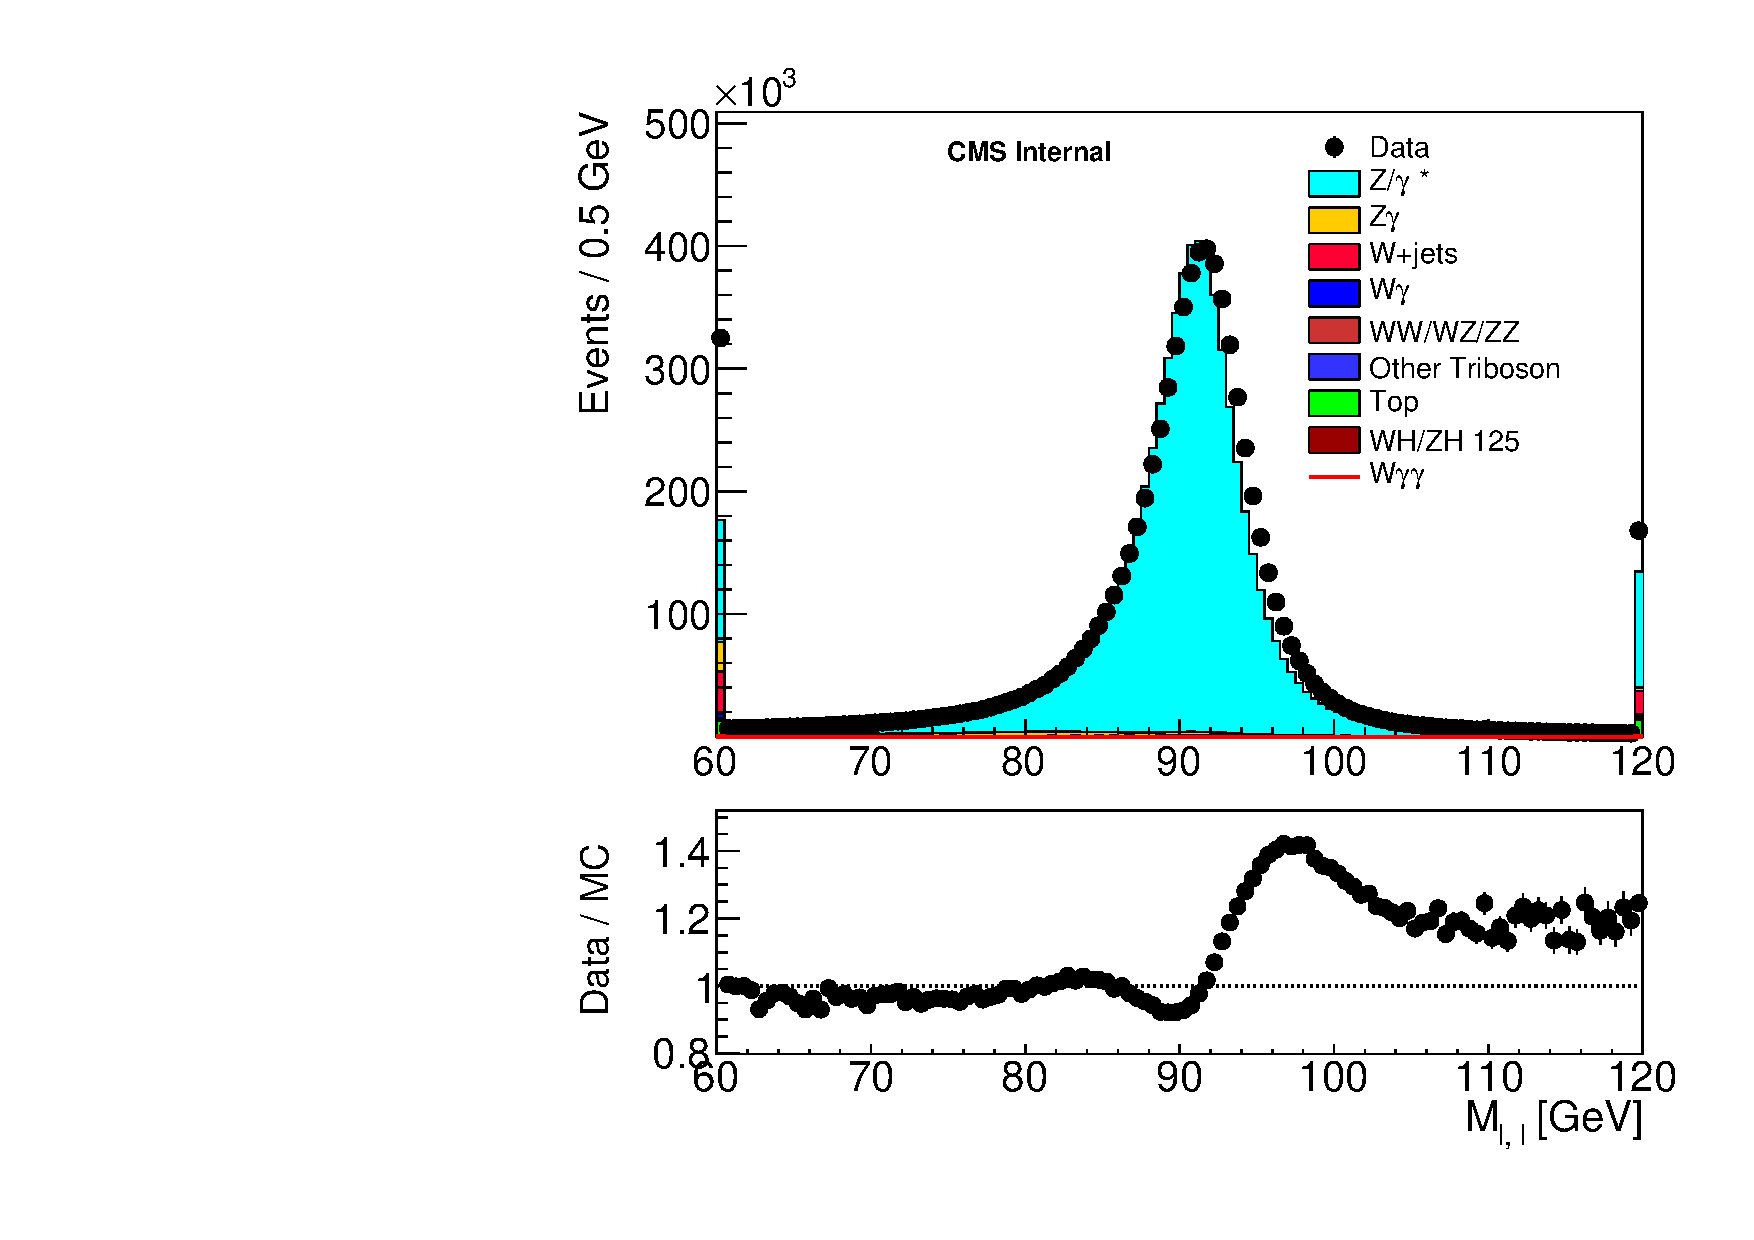
\includegraphics[width=0.6\textwidth]{Plots/m_leplep_ee_zMassZoom_NoCorr.pdf}

        After
           
        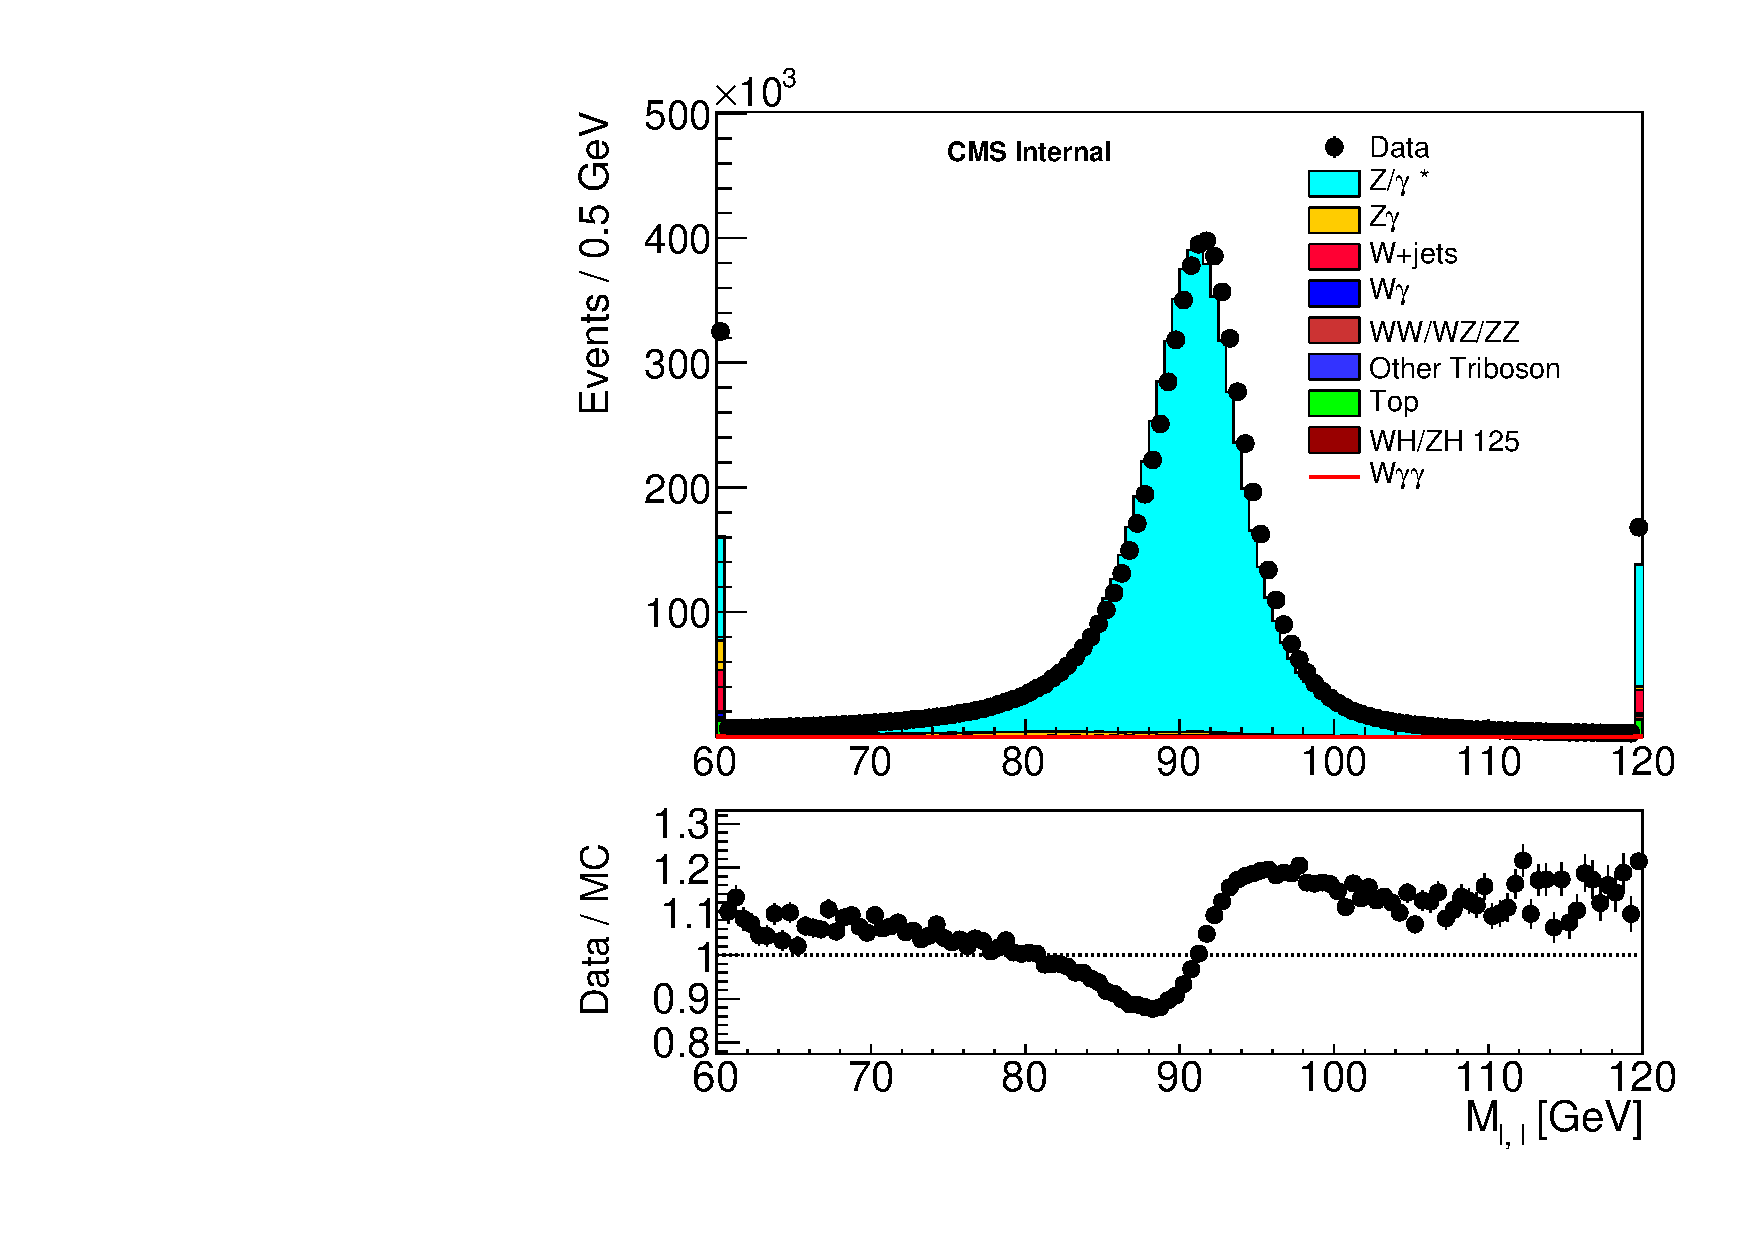
\includegraphics[width=0.6\textwidth]{Plots/m_leplep_ee_zMassZoom.pdf}

        \column{0.5\textwidth}
        Muons

        Before

        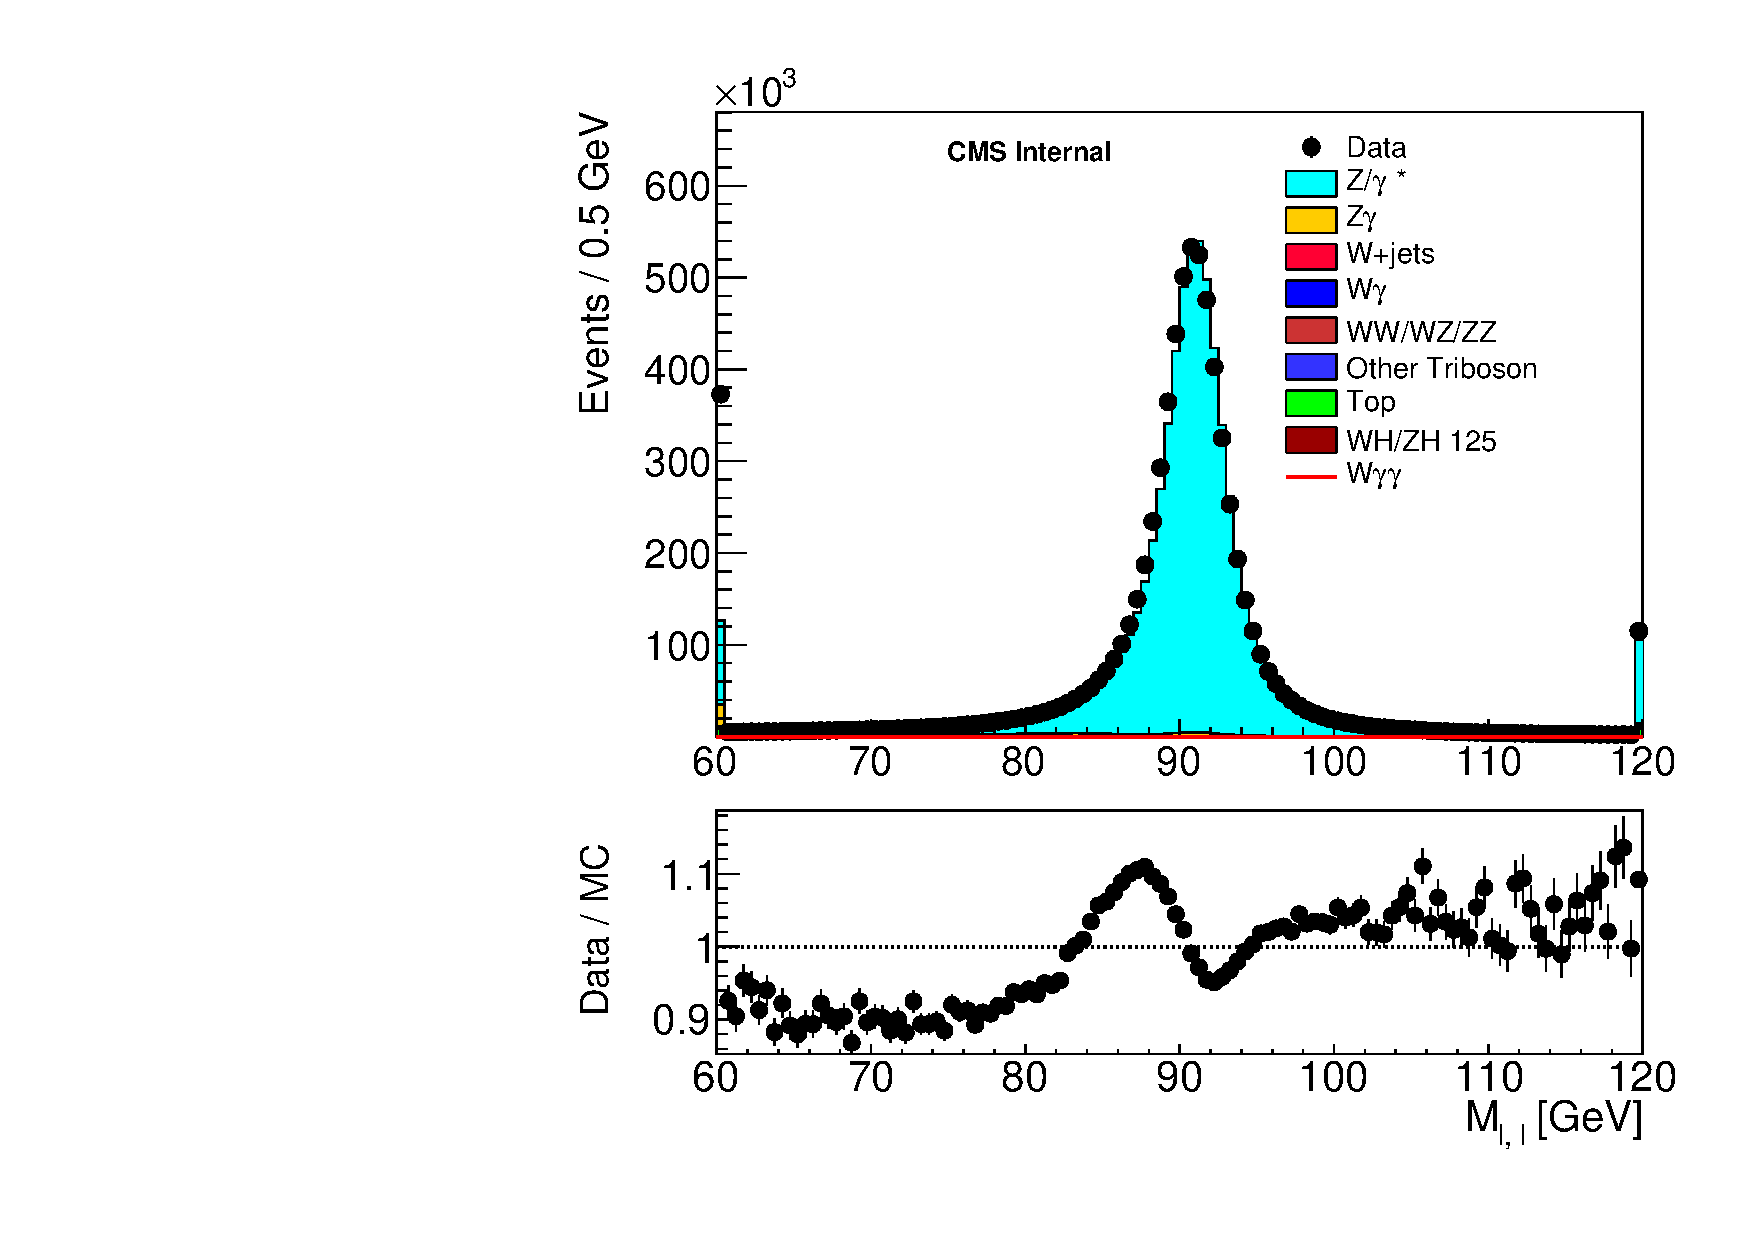
\includegraphics[width=0.6\textwidth]{Plots/m_leplep_mm_zMassZoom_NoCorr.pdf}

        After

        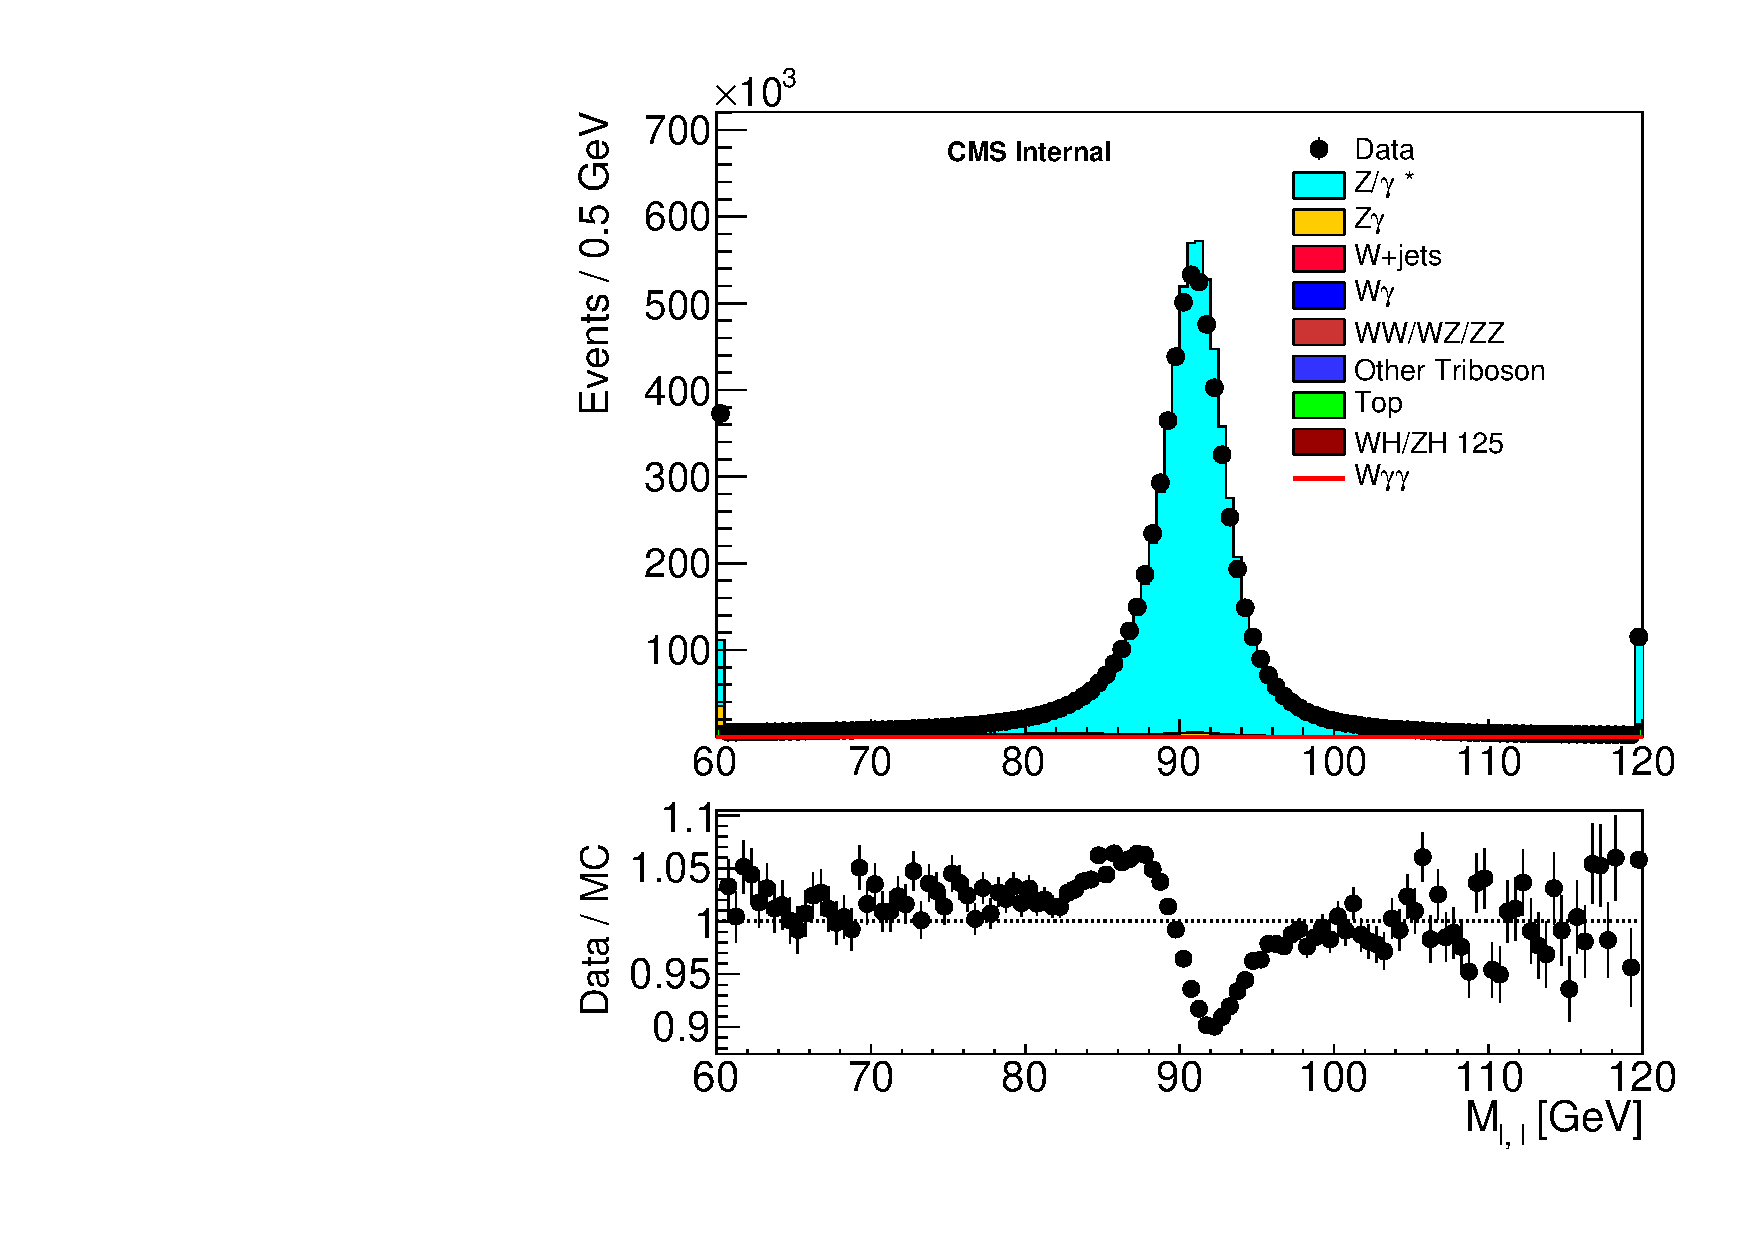
\includegraphics[width=0.6\textwidth]{Plots/m_leplep_mumu_zMassZoom.pdf}

    \ec


}

\fr{ Check corrected lepton momentum spectra } {

    Still about 10\% variation over the \pt spectrum


    \bc
        \column{0.5\textwidth}
        Electrons
   
        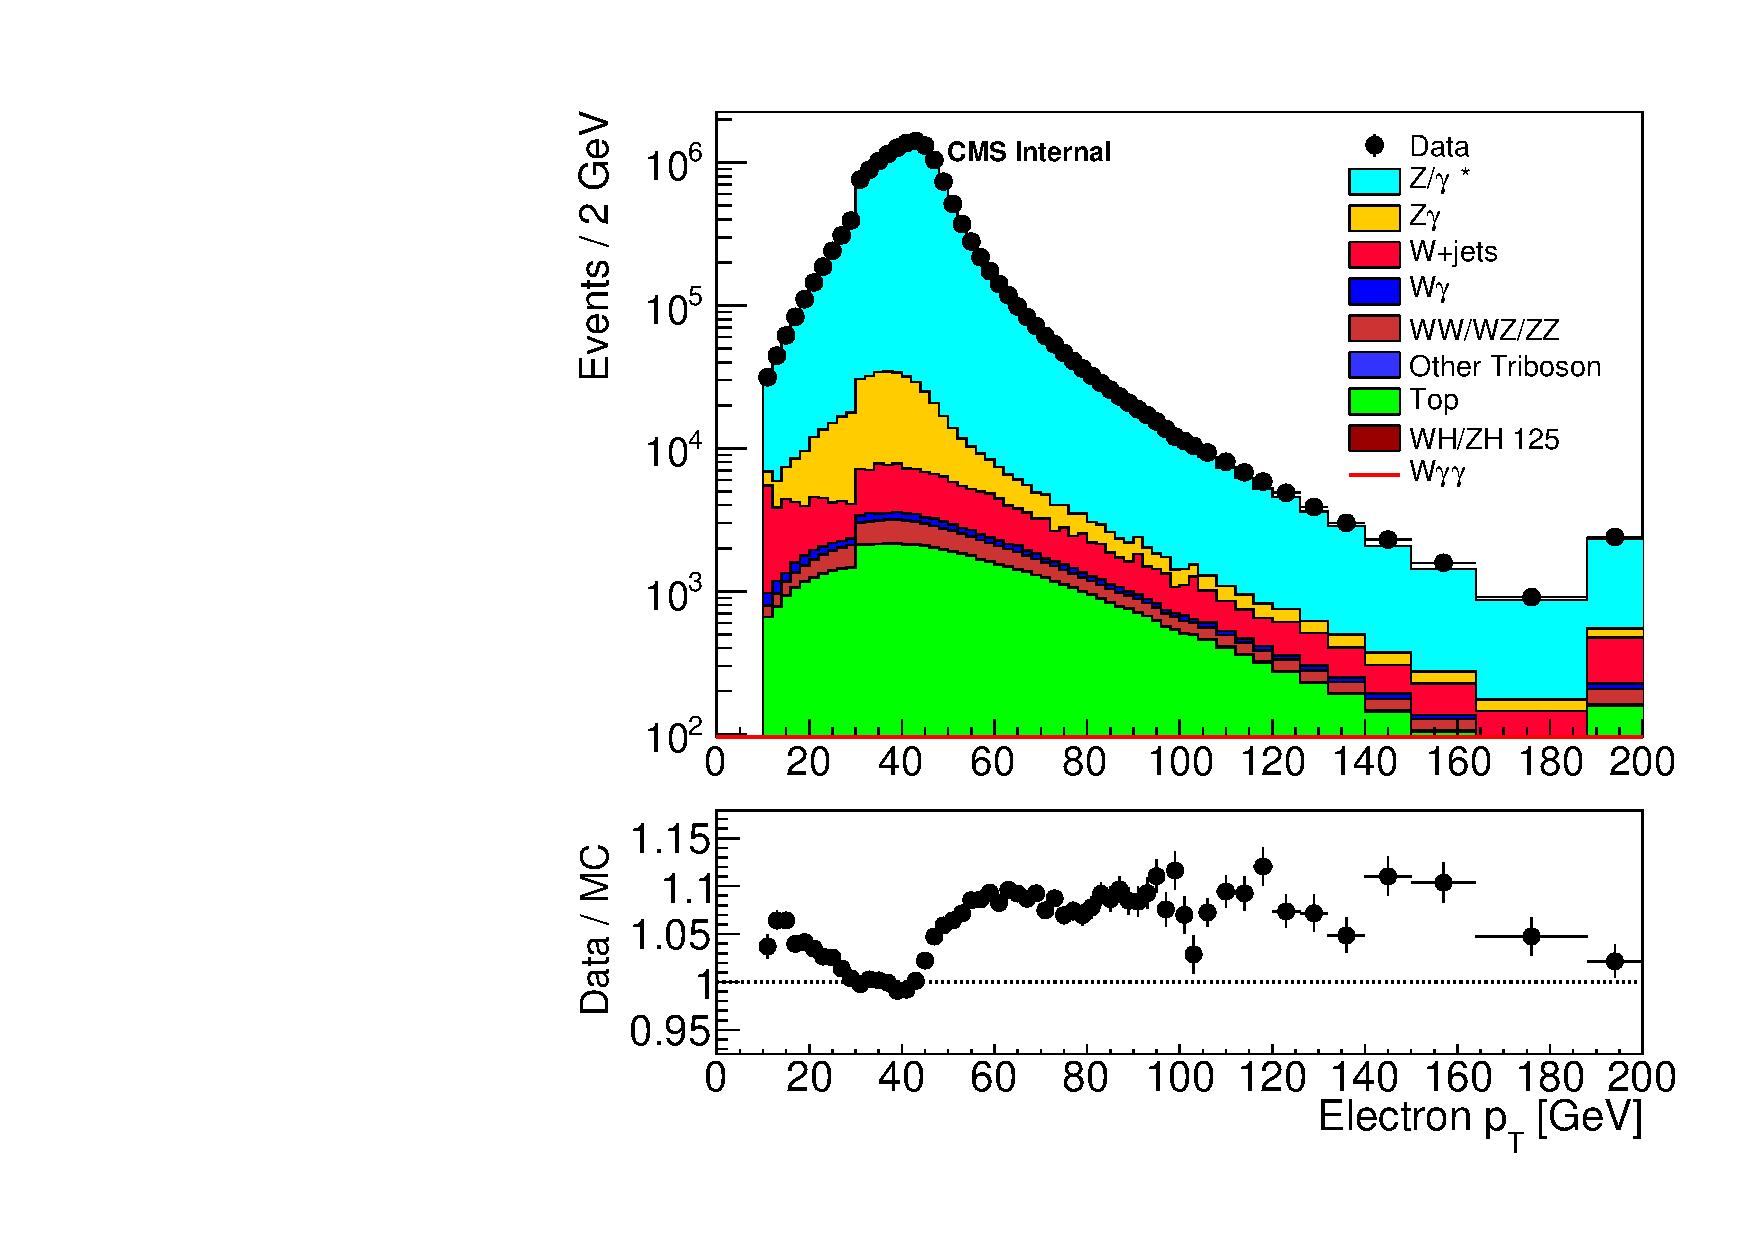
\includegraphics[width=0.8\textwidth]{Plots/mu_pt_ee_vetolowmass.pdf}

        \column{0.5\textwidth}
        Muons

        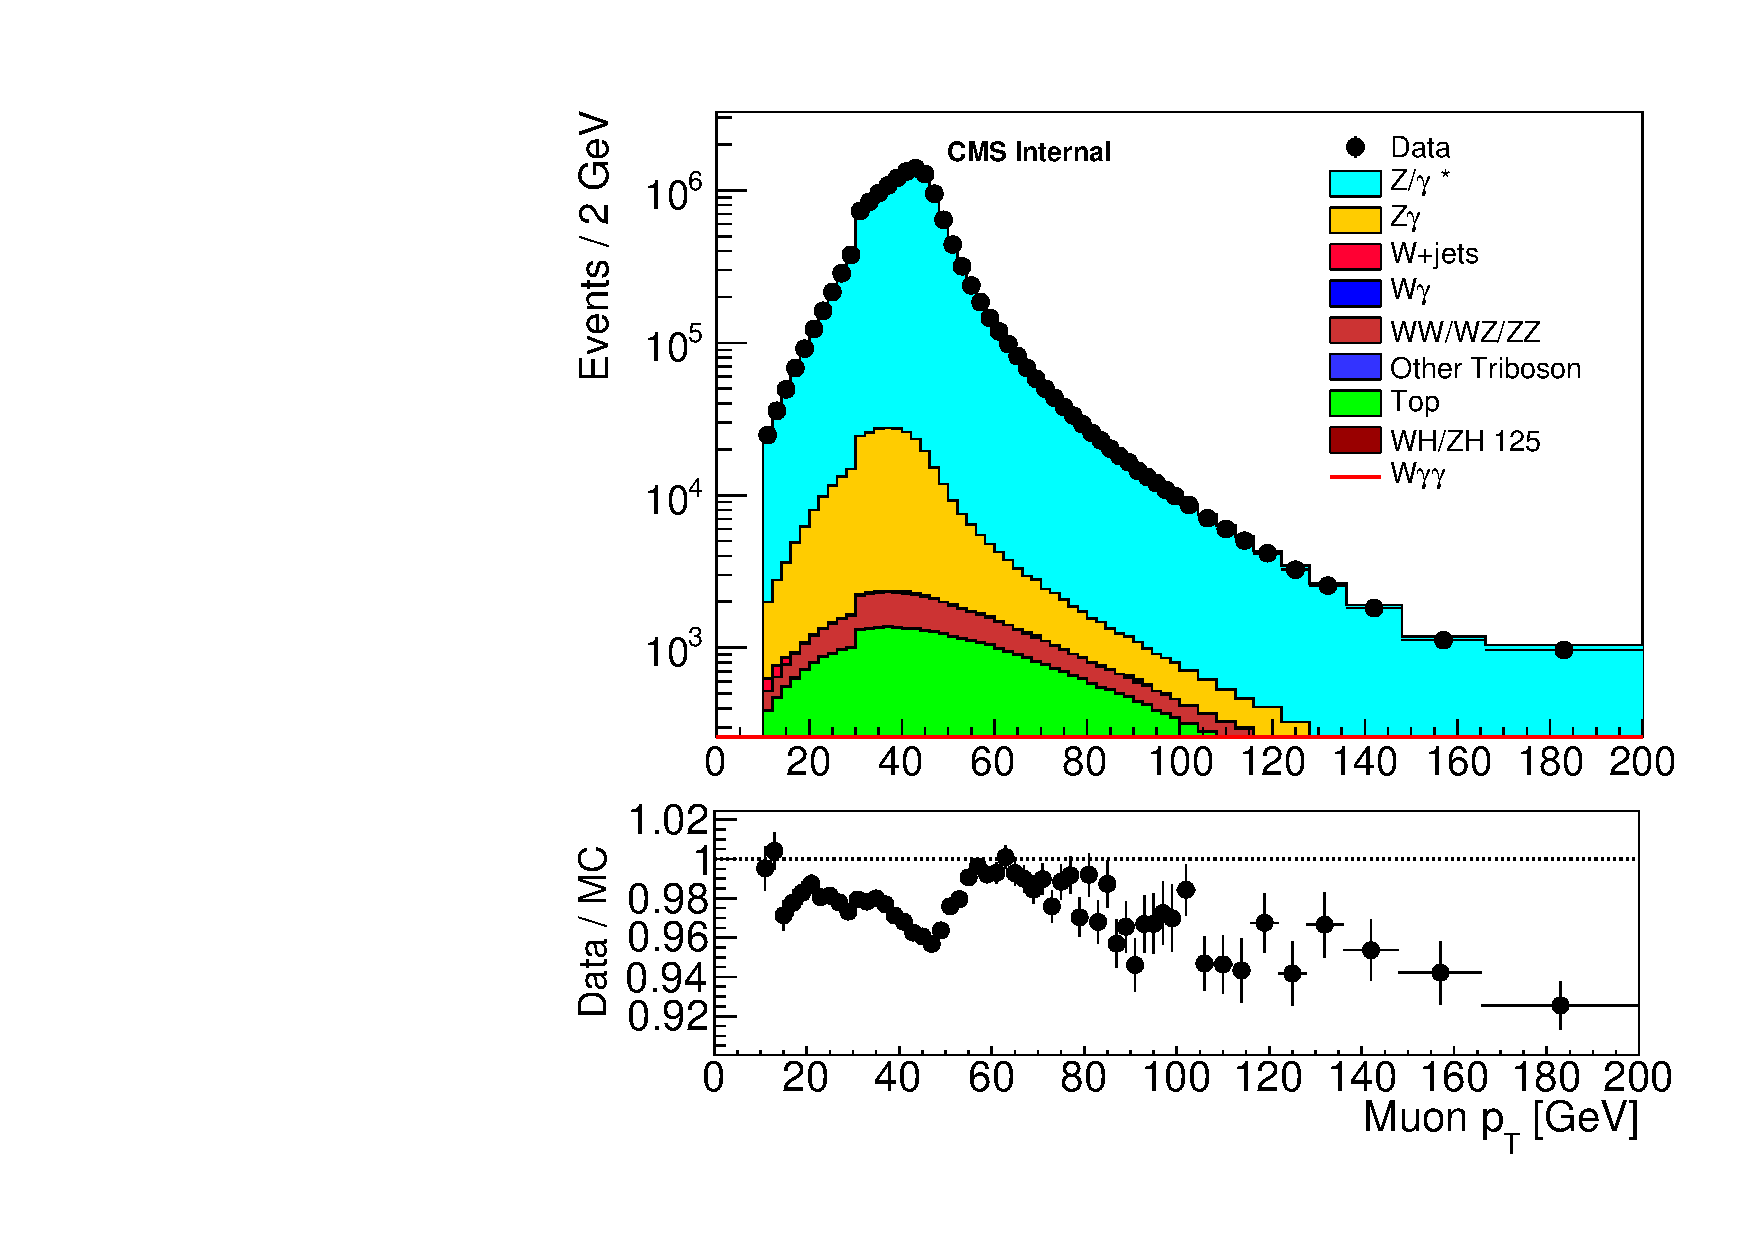
\includegraphics[width=0.8\textwidth]{Plots/mu_pt_mm_vetolowmass.pdf}

    \ec
}

\fr{ Second lepton veto } {

    Check efficiency of veto on additional leptons having $\pt > 10$ GeV

    \vspace{2mm}

    \bc
        \column{0.5\textwidth}
    \scriptsize
        Electron channel

        \begin{tabular}{| l l l l |}  \hline
                     & Total MC  & Signal & Signal / bkg \\ \hline
        Before       &  2563 & 338       &  0.13 \\
        After        &  2213 & 334       &  0.15 \\
        \end{tabular}

        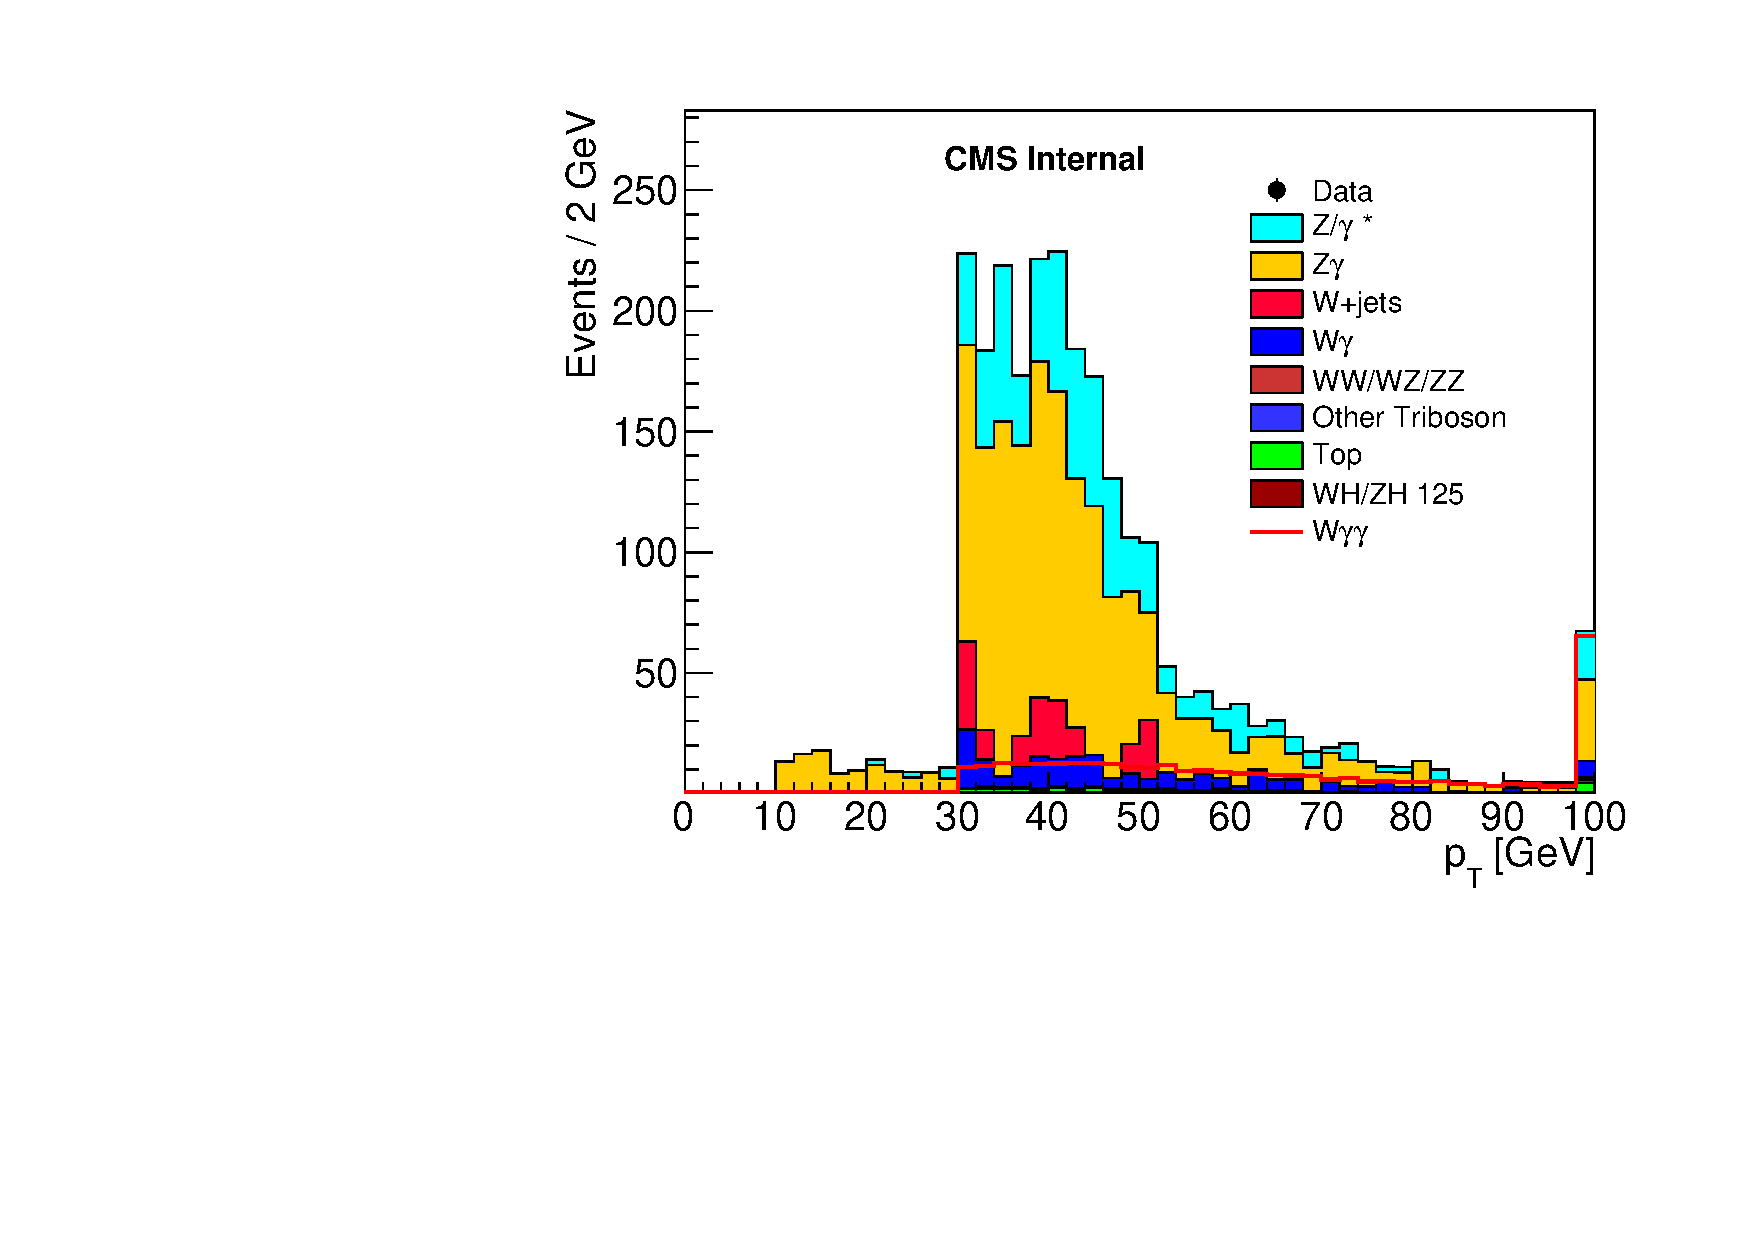
\includegraphics[width=0.8\textwidth]{Plots/el_pt_ephph_no2ndveto.pdf}

        \column{0.5\textwidth}

    \scriptsize

        \begin{tabular}{| l l l l |}  \hline
               & Total MC  & Signal & Signal / bkg \\ \hline
        Before & 1059      & 357    & 0.34             \\
        After  & 752       & 357    & 0.47              \\
        \end{tabular}

        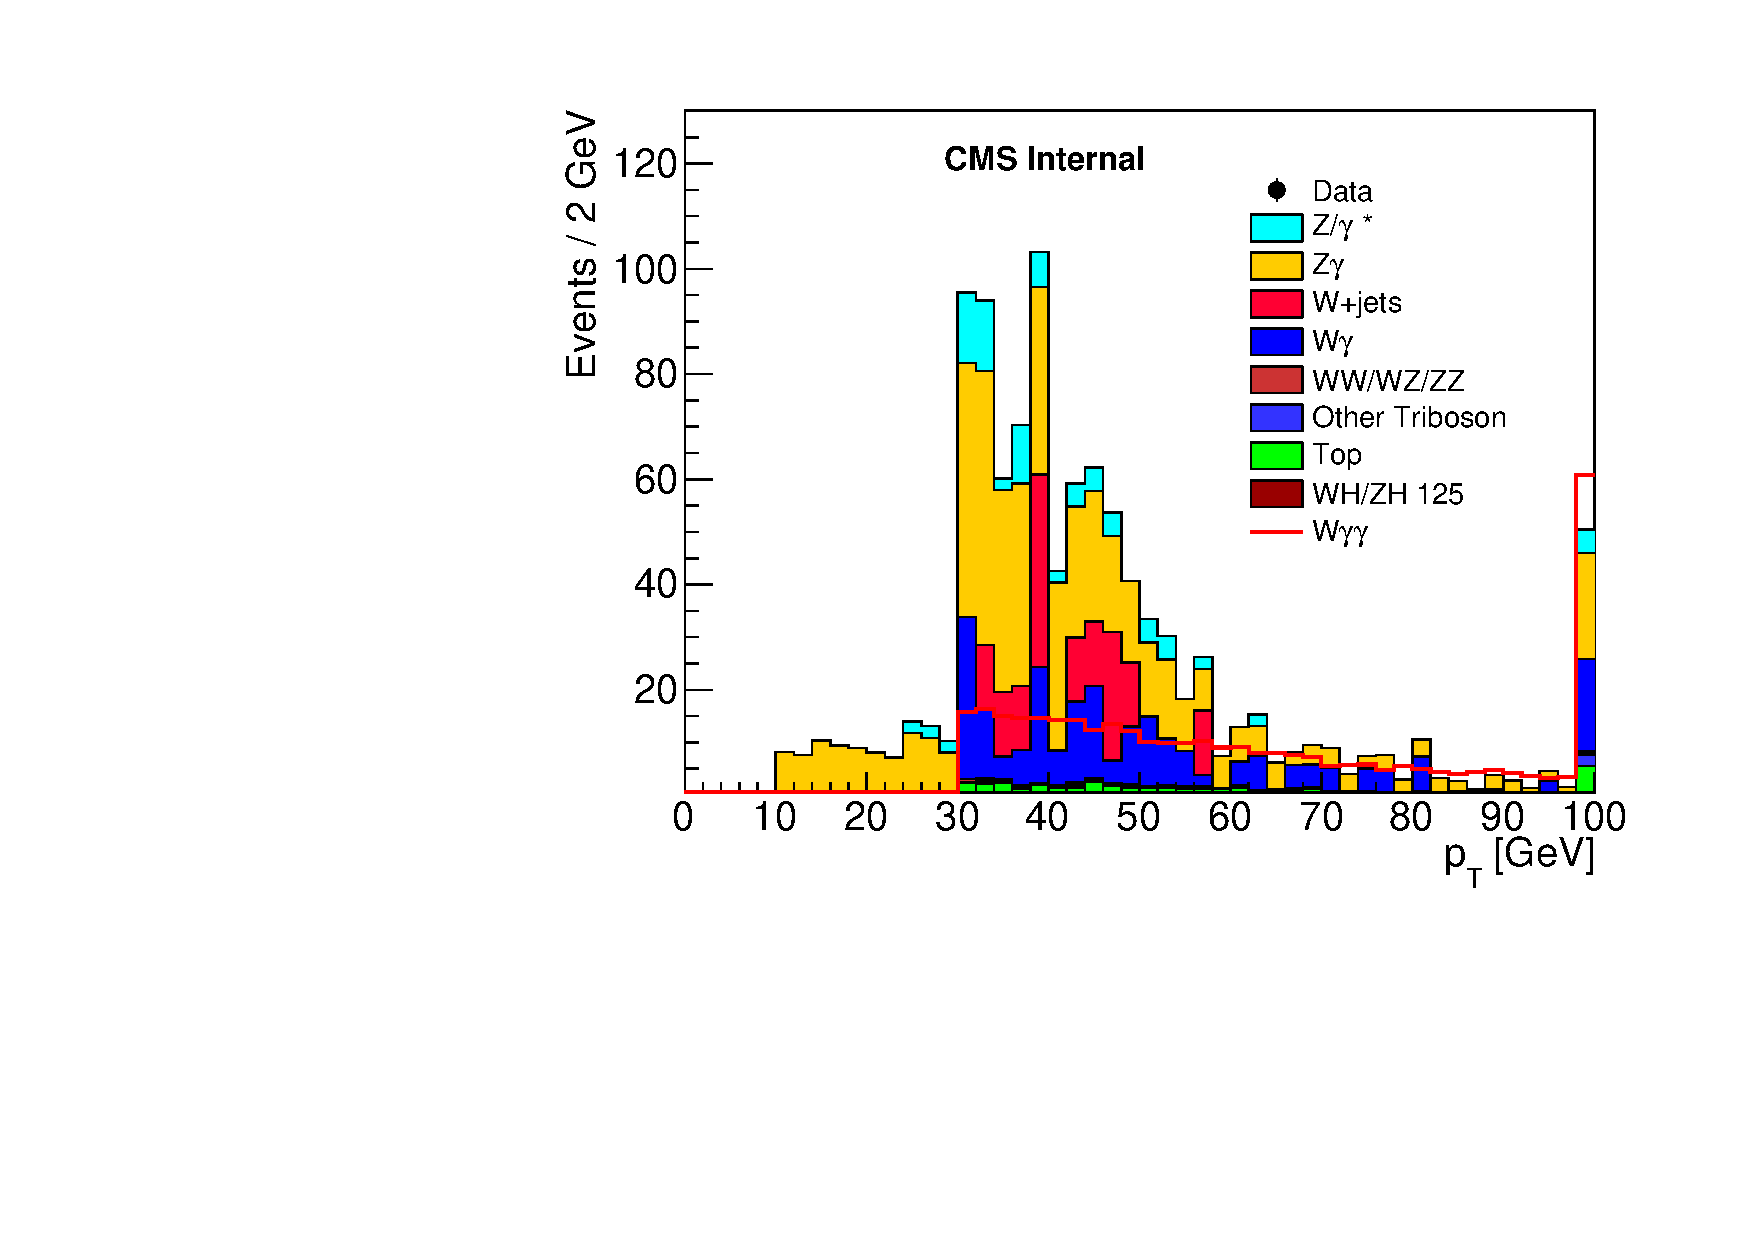
\includegraphics[width=0.8\textwidth]{Plots/mu_pt_mphph_no2ndveto.pdf}

    \ec
}


\fr{ Three photon events } {

    \scriptsize

    \begin{itemize}
        \item While our signal prefers to produce 2 photons, it is possible to emit an additional photon
        \item The number of events is small, but the requirement of a third photon further reduces background
        \item Could provide additional TGC/QGC sensitivity
        \item Unclear if we should include it in the cross section "what cross section are we measuring?"
        \item May present some challenges to background estimation
    \end{itemize}

    Muon channel
    
    \begin{tabular}{ | l l l l |}\hline
     & Total MC & Signal & Signal / bkg \\ \hline
        2 photons  & 752 & 357 &  0.15  \\
        3 photons  & 0.6 & 1.2 &  2  \\
        3 photons, 3rd photon $\pt > 10$ GeV & 3.1 & 4.2 &  1.35  \\
    \end{tabular}

    Electron channel

    \begin{tabular}{ | l l l l |}\hline
     & Total MC & Signal & Signal / bkg \\ \hline
        2 photons  & 2213 & 334 & 0.47   \\
        3 photons  & 3.5 & 1.8 &  0.51  \\
        3 photons, 3rd photon $\pt > 10$ GeV & 16.2 & 4.0 & 0.25  \\
    \end{tabular}

}

\end{document}

